\documentclass[preprint,12pt,authoryear]{elsarticle}
\usepackage{amsmath,amssymb}
\usepackage{graphicx}
\usepackage{booktabs}
\usepackage{siunitx}
\usepackage{hyperref}
\usepackage{xcolor}
\usepackage{array}
\usepackage[section]{placeins}
\graphicspath{{figures/}}
% Generated by launchcum.pipeline; do not edit by hand.
\newcommand{\valAreaExistingCdnlFiveFiveKmTwo}{1,701}
\newcommand{\valAreaExistingCdnlSixZeroKmTwo}{614}
\newcommand{\valAreaExistingCdnlSixFiveKmTwo}{226}
\newcommand{\valAreaExistingLdnFiveFiveKmTwo}{319}
\newcommand{\valAreaExistingLdnSixZeroKmTwo}{152}
\newcommand{\valAreaExistingLdnSixFiveKmTwo}{73.5}
\newcommand{\valAreaExistingLdnSevenZeroKmTwo}{38.0}
\newcommand{\valAreaPhaseOneCdnlFiveFiveKmTwo}{3,600}
\newcommand{\valAreaPhaseOneCdnlSixZeroKmTwo}{3,586}
\newcommand{\valAreaPhaseOneCdnlSixFiveKmTwo}{1,785}
\newcommand{\valAreaPhaseOneLdnFiveFiveKmTwo}{1,354}
\newcommand{\valAreaPhaseOneLdnSixZeroKmTwo}{678}
\newcommand{\valAreaPhaseOneLdnSixFiveKmTwo}{332}
\newcommand{\valAreaPhaseOneLdnSevenZeroKmTwo}{156}
\newcommand{\valAreaPhaseTwoCdnlFiveFiveKmTwo}{3,600}
\newcommand{\valAreaPhaseTwoCdnlSixZeroKmTwo}{3,600}
\newcommand{\valAreaPhaseTwoCdnlSixFiveKmTwo}{3,600}
\newcommand{\valAreaPhaseTwoFnZeroOneTwoCdnlFiveFiveKmTwo}{3,600}
\newcommand{\valAreaPhaseTwoFnZeroOneTwoCdnlSixZeroKmTwo}{3,600}
\newcommand{\valAreaPhaseTwoFnZeroOneTwoCdnlSixFiveKmTwo}{2,916}
\newcommand{\valAreaPhaseTwoFnZeroOneTwoLdnFiveFiveKmTwo}{1,860}
\newcommand{\valAreaPhaseTwoFnZeroOneTwoLdnSixZeroKmTwo}{941}
\newcommand{\valAreaPhaseTwoFnZeroOneTwoLdnSixFiveKmTwo}{470}
\newcommand{\valAreaPhaseTwoFnZeroOneTwoLdnSevenZeroKmTwo}{224}
\newcommand{\valAreaPhaseTwoLdnFiveFiveKmTwo}{2,984}
\newcommand{\valAreaPhaseTwoLdnSixZeroKmTwo}{1,682}
\newcommand{\valAreaPhaseTwoLdnSixFiveKmTwo}{846}
\newcommand{\valAreaPhaseTwoLdnSevenZeroKmTwo}{420}
\newcommand{\valBudgetPerLaunchTwoZeroZeroZeroNOneZeroZeroH}{20.0}
\newcommand{\valBudgetPerLaunchTwoZeroZeroZeroNFourFiveSixH}{4.39}
\newcommand{\valBudgetPerLaunchFiveZeroZeroNOneZeroZeroH}{5.00}
\newcommand{\valBudgetPerLaunchFiveZeroZeroNFourFiveSixH}{1.10}
\newcommand{\valBudgetPerLaunchEightZeroZeroNOneZeroZeroH}{8.00}
\newcommand{\valBudgetPerLaunchEightZeroZeroNFourFiveSixH}{1.75}
\newcommand{\valCfCountTermTwoFiveOneZeroZeroDb}{6.02}
\newcommand{\valCfCountTermTwoFiveFourFiveSixDb}{12.6}
\newcommand{\valCfNightTermZeroOneTwoZeroFiveDb}{4.22}
\newcommand{\valCfTotalTwoFiveOneZeroZeroDb}{10.2}
\newcommand{\valCfTotalTwoFiveFourFiveSixDb}{16.8}
\newcommand{\valConvCdnlSixZeroRel}{-1.29e-03}
\newcommand{\valConvDnlSixFiveRel}{8.13e-03}
\newcommand{\valConvPhaseTwoLdnSixFiveRel}{9.61e-04}
\newcommand{\valConvPhaseTwoMaxRel}{1.01e-03}
\newcommand{\valConvPhaseTwoMaxRelPct}{0.101}
\newcommand{\valEOneCoverageCfMaxabsdiff}{0.021}
\newcommand{\valEOneErrBoomTwoPortIsabelNearestEdge}{-2.44}
\newcommand{\valEOneErrClosureH}{2,673}
\newcommand{\valEOneErrDaysNineZeroPortIsabelNearestEdge}{456}
\newcommand{\valEOneErrDaysNineZeroSouthPadreIslandNearestEdge}{456}
\newcommand{\valEOneErrDelugeGal}{-1,197,482}
\newcommand{\valEOneErrDisturbedLowerRioGrandeValleyNwrNearPad}{8.92e-03}
\newcommand{\valEOneErrDisturbedPipingPloverCriticalHabitatNearPad}{8.23e-03}
\newcommand{\valEOneErrLdnPortIsabelNearestEdge}{-0.165}
\newcommand{\valEOneErrNaOneZeroZeroPortIsabelNearestEdge}{-1.18}
\newcommand{\valEOneErrNoxTons}{-4.61}
\newcommand{\valEOneExtBoomOnePortisabelZero}{911}
\newcommand{\valEOneExtBoomOnePortisabelOne}{1,367}
\newcommand{\valEOneExtDaysNineZeroSpiZero}{328}
\newcommand{\valEOneExtDaysNineZeroSpiOne}{354}
\newcommand{\valEOneExtLdnDeltaDb}{0.220}
\newcommand{\valEOneExtLdnPortisabelZero}{75.7}
\newcommand{\valEOneExtLdnPortisabelOne}{75.9}
\newcommand{\valEOneLinBoomTwoPortIsabelNearestEdge}{908}
\newcommand{\valEOneLinClosureH}{7,993}
\newcommand{\valEOneLinDaysNineZeroPortIsabelNearestEdge}{784}
\newcommand{\valEOneLinDaysNineZeroSouthPadreIslandNearestEdge}{784}
\newcommand{\valEOneLinDelugeGal}{421,569,249}
\newcommand{\valEOneLinDisturbedLowerRioGrandeValleyNwrNearPad}{0.142}
\newcommand{\valEOneLinDisturbedPipingPloverCriticalHabitatNearPad}{0.141}
\newcommand{\valEOneLinLdnPortIsabelNearestEdge}{75.5}
\newcommand{\valEOneLinNaOneZeroZeroPortIsabelNearestEdge}{455}
\newcommand{\valEOneLinNoxTons}{1,691}
\newcommand{\valEOneNOneZeroZeroBoomTwoPortisabel}{200}
\newcommand{\valEOneNOneZeroZeroClosureH}{1,627}
\newcommand{\valEOneNOneZeroZeroDaysNineZeroSpi}{144}
\newcommand{\valEOneNOneZeroZeroDisturbedHabitat}{0.031}
\newcommand{\valEOneNOneZeroZeroLdnPortisabel}{69.0}
\newcommand{\valEOneNOneZeroZeroNaOneZeroZeroPortisabel}{100}
\newcommand{\valEOneNOneZeroZeroSummerAvail}{0.799}
\newcommand{\valEOneNOneZeroZeroWeekendAvail}{0.800}
\newcommand{\valEOneNTwoZeroZeroBoomTwoPortisabel}{399}
\newcommand{\valEOneNTwoZeroZeroClosureH}{2,949}
\newcommand{\valEOneNTwoZeroZeroDaysNineZeroSpi}{231}
\newcommand{\valEOneNTwoZeroZeroDisturbedHabitat}{0.061}
\newcommand{\valEOneNTwoZeroZeroLdnPortisabel}{72.1}
\newcommand{\valEOneNTwoZeroZeroNaOneZeroZeroPortisabel}{200}
\newcommand{\valEOneNTwoZeroZeroSummerAvail}{0.639}
\newcommand{\valEOneNTwoZeroZeroWeekendAvail}{0.640}
\newcommand{\valEOneNTwoFiveBoomTwoPortisabel}{49.8}
\newcommand{\valEOneNTwoFiveClosureH}{438}
\newcommand{\valEOneNTwoFiveDaysNineZeroSpi}{43.0}
\newcommand{\valEOneNTwoFiveDisturbedHabitat}{7.74e-03}
\newcommand{\valEOneNTwoFiveLdnPortisabel}{62.9}
\newcommand{\valEOneNTwoFiveNaOneZeroZeroPortisabel}{24.9}
\newcommand{\valEOneNTwoFiveSummerAvail}{0.946}
\newcommand{\valEOneNTwoFiveWeekendAvail}{0.946}
\newcommand{\valEOneNFourFiveSixBoomTwoPortisabel}{911}
\newcommand{\valEOneNFourFiveSixClosureH}{5,320}
\newcommand{\valEOneNFourFiveSixDaysNineZeroSpi}{328}
\newcommand{\valEOneNFourFiveSixDisturbedHabitat}{0.133}
\newcommand{\valEOneNFourFiveSixLdnPortisabel}{75.7}
\newcommand{\valEOneNFourFiveSixNaOneZeroZeroPortisabel}{456}
\newcommand{\valEOneNFourFiveSixSummerAvail}{0.361}
\newcommand{\valEOneNFourFiveSixWeekendAvail}{0.362}
\newcommand{\valEOneNFiveZeroBoomTwoPortisabel}{99.9}
\newcommand{\valEOneNFiveZeroClosureH}{855}
\newcommand{\valEOneNFiveZeroDaysNineZeroSpi}{81.2}
\newcommand{\valEOneNFiveZeroDisturbedHabitat}{0.016}
\newcommand{\valEOneNFiveZeroLdnPortisabel}{66.0}
\newcommand{\valEOneNFiveZeroNaOneZeroZeroPortisabel}{50.0}
\newcommand{\valEOneNFiveZeroSummerAvail}{0.894}
\newcommand{\valEOneNFiveZeroWeekendAvail}{0.894}
\newcommand{\valEOneRelerrBoomTwoPortIsabelNearestEdge}{-2.68e-03}
\newcommand{\valEOneRelerrClosureH}{0.502}
\newcommand{\valEOneRelerrDaysNineZeroPortIsabelNearestEdge}{1.39}
\newcommand{\valEOneRelerrDaysNineZeroSouthPadreIslandNearestEdge}{1.39}
\newcommand{\valEOneRelerrDelugeGal}{-2.83e-03}
\newcommand{\valEOneRelerrDisturbedLowerRioGrandeValleyNwrNearPad}{0.067}
\newcommand{\valEOneRelerrDisturbedPipingPloverCriticalHabitatNearPad}{0.062}
\newcommand{\valEOneRelerrLdnPortIsabelNearestEdge}{n/a}
\newcommand{\valEOneRelerrNaOneZeroZeroPortIsabelNearestEdge}{-2.59e-03}
\newcommand{\valEOneRelerrNoxTons}{-2.72e-03}
\newcommand{\valEOneRelerrPctBoomTwoPortIsabelNearestEdge}{-0.268}
\newcommand{\valEOneRelerrPctClosureH}{50.2}
\newcommand{\valEOneRelerrPctDaysNineZeroPortIsabelNearestEdge}{139}
\newcommand{\valEOneRelerrPctDaysNineZeroSouthPadreIslandNearestEdge}{139}
\newcommand{\valEOneRelerrPctDelugeGal}{-0.283}
\newcommand{\valEOneRelerrPctDisturbedLowerRioGrandeValleyNwrNearPad}{6.71}
\newcommand{\valEOneRelerrPctDisturbedPipingPloverCriticalHabitatNearPad}{6.19}
\newcommand{\valEOneRelerrPctNaOneZeroZeroPortIsabelNearestEdge}{-0.259}
\newcommand{\valEOneRelerrPctNoxTons}{-0.272}
\newcommand{\valEOneRelerrPctPctBoomTwoPortIsabelNearestEdge}{-26.8}
\newcommand{\valEOneRelerrPctPctClosureH}{5,024}
\newcommand{\valEOneRelerrPctPctDaysNineZeroPortIsabelNearestEdge}{13,912}
\newcommand{\valEOneRelerrPctPctDaysNineZeroSouthPadreIslandNearestEdge}{13,912}
\newcommand{\valEOneRelerrPctPctDelugeGal}{-28.3}
\newcommand{\valEOneRelerrPctPctDisturbedLowerRioGrandeValleyNwrNearPad}{671}
\newcommand{\valEOneRelerrPctPctDisturbedPipingPloverCriticalHabitatNearPad}{619}
\newcommand{\valEOneRelerrPctPctNaOneZeroZeroPortIsabelNearestEdge}{-25.9}
\newcommand{\valEOneRelerrPctPctNoxTons}{-27.2}
\newcommand{\valEOneRelerrPctPctPctBoomTwoPortIsabelNearestEdge}{-2,680}
\newcommand{\valEOneRelerrPctPctPctClosureH}{502,367}
\newcommand{\valEOneRelerrPctPctPctDaysNineZeroPortIsabelNearestEdge}{1,391,174}
\newcommand{\valEOneRelerrPctPctPctDaysNineZeroSouthPadreIslandNearestEdge}{1,391,174}
\newcommand{\valEOneRelerrPctPctPctDelugeGal}{-2,832}
\newcommand{\valEOneRelerrPctPctPctDisturbedLowerRioGrandeValleyNwrNearPad}{67,132}
\newcommand{\valEOneRelerrPctPctPctDisturbedPipingPloverCriticalHabitatNearPad}{61,928}
\newcommand{\valEOneRelerrPctPctPctNaOneZeroZeroPortIsabelNearestEdge}{-2,588}
\newcommand{\valEOneRelerrPctPctPctNoxTons}{-2,720}
\newcommand{\valEOneSimBoomTwoPortIsabelNearestEdge}{911}
\newcommand{\valEOneSimClosureH}{5,320}
\newcommand{\valEOneSimDaysNineZeroPortIsabelNearestEdge}{328}
\newcommand{\valEOneSimDaysNineZeroSouthPadreIslandNearestEdge}{328}
\newcommand{\valEOneSimDelugeGal}{422,766,732}
\newcommand{\valEOneSimDisturbedLowerRioGrandeValleyNwrNearPad}{0.133}
\newcommand{\valEOneSimDisturbedPipingPloverCriticalHabitatNearPad}{0.133}
\newcommand{\valEOneSimLdnPortIsabelNearestEdge}{75.7}
\newcommand{\valEOneSimNaOneZeroZeroPortIsabelNearestEdge}{456}
\newcommand{\valEOneSimNoxTons}{1,696}
\newcommand{\valETwoCampaignDaysNineZeroSpi}{257}
\newcommand{\valETwoCampaignDisturbedHabitat}{0.129}
\newcommand{\valETwoCampaignFeasible}{1.00}
\newcommand{\valETwoCampaignHasWindowHabitat}{1.00}
\newcommand{\valETwoCampaignLongestGapHabitatH}{266}
\newcommand{\valETwoCampaignSummerAvail}{0.473}
\newcommand{\valETwoCampaignWeekendAvail}{0.653}
\newcommand{\valETwoPoissonDaysNineZeroSpi}{328}
\newcommand{\valETwoPoissonDisturbedHabitat}{0.133}
\newcommand{\valETwoPoissonFeasible}{1.00}
\newcommand{\valETwoPoissonHasWindowHabitat}{1.00}
\newcommand{\valETwoPoissonLongestGapHabitatH}{70.7}
\newcommand{\valETwoPoissonSummerAvail}{0.361}
\newcommand{\valETwoPoissonWeekendAvail}{0.361}
\newcommand{\valETwoWeekdayDaysNineZeroSpi}{310}
\newcommand{\valETwoWeekdayDisturbedHabitat}{0.149}
\newcommand{\valETwoWeekdayFeasible}{1.00}
\newcommand{\valETwoWeekdayHasWindowHabitat}{1.00}
\newcommand{\valETwoWeekdayLongestGapHabitatH}{54.7}
\newcommand{\valETwoWeekdaySummerAvail}{0.322}
\newcommand{\valETwoWeekdayWeekendAvail}{0.625}
\newcommand{\valEThreeNaOneZeroZeroNightPortisabelFnZeroZero}{0}
\newcommand{\valEThreeNaOneZeroZeroNightPortisabelFnOneTwo}{54.7}
\newcommand{\valEThreeNaOneZeroZeroNightPortisabelFnFiveZero}{228}
\newcommand{\valEThreeNightCfMaxabsdiffDb}{0.191}
\newcommand{\valEFourExpectedUpperTwoZeroHNOneZeroZeroClosureH}{2,335}
\newcommand{\valEFourExpectedUpperTwoZeroHNOneZeroZeroPexceedTwoZeroZeroZero}{0.932}
\newcommand{\valEFourExpectedUpperTwoZeroHNOneZeroZeroPexceedFiveZeroZero}{1.00}
\newcommand{\valEFourExpectedUpperTwoZeroHNOneZeroZeroPexceedEightZeroZero}{1.00}
\newcommand{\valEFourExpectedUpperTwoZeroHNOneZeroZeroSummerAvail}{0.727}
\newcommand{\valEFourExpectedUpperTwoZeroHNOneZeroZeroWeekendAvail}{0.728}
\newcommand{\valEFourExpectedUpperTwoZeroHNTwoZeroZeroClosureH}{4,095}
\newcommand{\valEFourExpectedUpperTwoZeroHNTwoZeroZeroPexceedTwoZeroZeroZero}{1.00}
\newcommand{\valEFourExpectedUpperTwoZeroHNTwoZeroZeroPexceedFiveZeroZero}{1.00}
\newcommand{\valEFourExpectedUpperTwoZeroHNTwoZeroZeroPexceedEightZeroZero}{1.00}
\newcommand{\valEFourExpectedUpperTwoZeroHNTwoZeroZeroSummerAvail}{0.529}
\newcommand{\valEFourExpectedUpperTwoZeroHNTwoZeroZeroWeekendAvail}{0.531}
\newcommand{\valEFourExpectedUpperTwoZeroHNTwoFiveClosureH}{647}
\newcommand{\valEFourExpectedUpperTwoZeroHNTwoFivePexceedTwoZeroZeroZero}{0}
\newcommand{\valEFourExpectedUpperTwoZeroHNTwoFivePexceedFiveZeroZero}{0.856}
\newcommand{\valEFourExpectedUpperTwoZeroHNTwoFivePexceedEightZeroZero}{0.135}
\newcommand{\valEFourExpectedUpperTwoZeroHNTwoFiveSummerAvail}{0.924}
\newcommand{\valEFourExpectedUpperTwoZeroHNTwoFiveWeekendAvail}{0.924}
\newcommand{\valEFourExpectedUpperTwoZeroHNFourFiveSixClosureH}{6,914}
\newcommand{\valEFourExpectedUpperTwoZeroHNFourFiveSixPexceedTwoZeroZeroZero}{1.00}
\newcommand{\valEFourExpectedUpperTwoZeroHNFourFiveSixPexceedFiveZeroZero}{1.00}
\newcommand{\valEFourExpectedUpperTwoZeroHNFourFiveSixPexceedEightZeroZero}{1.00}
\newcommand{\valEFourExpectedUpperTwoZeroHNFourFiveSixSummerAvail}{0.235}
\newcommand{\valEFourExpectedUpperTwoZeroHNFourFiveSixWeekendAvail}{0.236}
\newcommand{\valEFourExpectedUpperTwoZeroHNFiveZeroClosureH}{1,248}
\newcommand{\valEFourExpectedUpperTwoZeroHNFiveZeroPexceedTwoZeroZeroZero}{1.00e-04}
\newcommand{\valEFourExpectedUpperTwoZeroHNFiveZeroPexceedFiveZeroZero}{1.00}
\newcommand{\valEFourExpectedUpperTwoZeroHNFiveZeroPexceedEightZeroZero}{0.995}
\newcommand{\valEFourExpectedUpperTwoZeroHNFiveZeroSummerAvail}{0.853}
\newcommand{\valEFourExpectedUpperTwoZeroHNFiveZeroWeekendAvail}{0.853}
\newcommand{\valEFourRecentFlightsTwoToFourNOneZeroZeroClosureH}{1,361}
\newcommand{\valEFourRecentFlightsTwoToFourNOneZeroZeroPexceedTwoZeroZeroZero}{0}
\newcommand{\valEFourRecentFlightsTwoToFourNOneZeroZeroPexceedFiveZeroZero}{1.00}
\newcommand{\valEFourRecentFlightsTwoToFourNOneZeroZeroPexceedEightZeroZero}{1.000}
\newcommand{\valEFourRecentFlightsTwoToFourNOneZeroZeroSummerAvail}{0.842}
\newcommand{\valEFourRecentFlightsTwoToFourNOneZeroZeroWeekendAvail}{0.843}
\newcommand{\valEFourRecentFlightsTwoToFourNTwoZeroZeroClosureH}{2,539}
\newcommand{\valEFourRecentFlightsTwoToFourNTwoZeroZeroPexceedTwoZeroZeroZero}{0.999}
\newcommand{\valEFourRecentFlightsTwoToFourNTwoZeroZeroPexceedFiveZeroZero}{1.00}
\newcommand{\valEFourRecentFlightsTwoToFourNTwoZeroZeroPexceedEightZeroZero}{1.00}
\newcommand{\valEFourRecentFlightsTwoToFourNTwoZeroZeroSummerAvail}{0.709}
\newcommand{\valEFourRecentFlightsTwoToFourNTwoZeroZeroWeekendAvail}{0.710}
\newcommand{\valEFourRecentFlightsTwoToFourNTwoFiveClosureH}{359}
\newcommand{\valEFourRecentFlightsTwoToFourNTwoFivePexceedTwoZeroZeroZero}{0}
\newcommand{\valEFourRecentFlightsTwoToFourNTwoFivePexceedFiveZeroZero}{0.051}
\newcommand{\valEFourRecentFlightsTwoToFourNTwoFivePexceedEightZeroZero}{0}
\newcommand{\valEFourRecentFlightsTwoToFourNTwoFiveSummerAvail}{0.958}
\newcommand{\valEFourRecentFlightsTwoToFourNTwoFiveWeekendAvail}{0.958}
\newcommand{\valEFourRecentFlightsTwoToFourNFourFiveSixClosureH}{4,885}
\newcommand{\valEFourRecentFlightsTwoToFourNFourFiveSixPexceedTwoZeroZeroZero}{1.00}
\newcommand{\valEFourRecentFlightsTwoToFourNFourFiveSixPexceedFiveZeroZero}{1.00}
\newcommand{\valEFourRecentFlightsTwoToFourNFourFiveSixPexceedEightZeroZero}{1.00}
\newcommand{\valEFourRecentFlightsTwoToFourNFourFiveSixSummerAvail}{0.458}
\newcommand{\valEFourRecentFlightsTwoToFourNFourFiveSixWeekendAvail}{0.459}
\newcommand{\valEFourRecentFlightsTwoToFourNFiveZeroClosureH}{705}
\newcommand{\valEFourRecentFlightsTwoToFourNFiveZeroPexceedTwoZeroZeroZero}{0}
\newcommand{\valEFourRecentFlightsTwoToFourNFiveZeroPexceedFiveZeroZero}{0.977}
\newcommand{\valEFourRecentFlightsTwoToFourNFiveZeroPexceedEightZeroZero}{0.192}
\newcommand{\valEFourRecentFlightsTwoToFourNFiveZeroSummerAvail}{0.918}
\newcommand{\valEFourRecentFlightsTwoToFourNFiveZeroWeekendAvail}{0.918}
\newcommand{\valEFourRecordFlightsOneToFourNOneZeroZeroClosureH}{1,720}
\newcommand{\valEFourRecordFlightsOneToFourNOneZeroZeroPexceedTwoZeroZeroZero}{0.068}
\newcommand{\valEFourRecordFlightsOneToFourNOneZeroZeroPexceedFiveZeroZero}{1.00}
\newcommand{\valEFourRecordFlightsOneToFourNOneZeroZeroPexceedEightZeroZero}{1.00}
\newcommand{\valEFourRecordFlightsOneToFourNOneZeroZeroSummerAvail}{0.799}
\newcommand{\valEFourRecordFlightsOneToFourNOneZeroZeroWeekendAvail}{0.800}
\newcommand{\valEFourRecordFlightsOneToFourNTwoZeroZeroClosureH}{3,143}
\newcommand{\valEFourRecordFlightsOneToFourNTwoZeroZeroPexceedTwoZeroZeroZero}{1.00}
\newcommand{\valEFourRecordFlightsOneToFourNTwoZeroZeroPexceedFiveZeroZero}{1.00}
\newcommand{\valEFourRecordFlightsOneToFourNTwoZeroZeroPexceedEightZeroZero}{1.00}
\newcommand{\valEFourRecordFlightsOneToFourNTwoZeroZeroSummerAvail}{0.639}
\newcommand{\valEFourRecordFlightsOneToFourNTwoZeroZeroWeekendAvail}{0.640}
\newcommand{\valEFourRecordFlightsOneToFourNTwoFiveClosureH}{463}
\newcommand{\valEFourRecordFlightsOneToFourNTwoFivePexceedTwoZeroZeroZero}{0}
\newcommand{\valEFourRecordFlightsOneToFourNTwoFivePexceedFiveZeroZero}{0.350}
\newcommand{\valEFourRecordFlightsOneToFourNTwoFivePexceedEightZeroZero}{2.20e-03}
\newcommand{\valEFourRecordFlightsOneToFourNTwoFiveSummerAvail}{0.945}
\newcommand{\valEFourRecordFlightsOneToFourNTwoFiveWeekendAvail}{0.946}
\newcommand{\valEFourRecordFlightsOneToFourNFourFiveSixClosureH}{5,757}
\newcommand{\valEFourRecordFlightsOneToFourNFourFiveSixPexceedTwoZeroZeroZero}{1.00}
\newcommand{\valEFourRecordFlightsOneToFourNFourFiveSixPexceedFiveZeroZero}{1.00}
\newcommand{\valEFourRecordFlightsOneToFourNFourFiveSixPexceedEightZeroZero}{1.00}
\newcommand{\valEFourRecordFlightsOneToFourNFourFiveSixSummerAvail}{0.360}
\newcommand{\valEFourRecordFlightsOneToFourNFourFiveSixWeekendAvail}{0.362}
\newcommand{\valEFourRecordFlightsOneToFourNFiveZeroClosureH}{903}
\newcommand{\valEFourRecordFlightsOneToFourNFiveZeroPexceedTwoZeroZeroZero}{0}
\newcommand{\valEFourRecordFlightsOneToFourNFiveZeroPexceedFiveZeroZero}{0.999}
\newcommand{\valEFourRecordFlightsOneToFourNFiveZeroPexceedEightZeroZero}{0.758}
\newcommand{\valEFourRecordFlightsOneToFourNFiveZeroSummerAvail}{0.894}
\newcommand{\valEFourRecordFlightsOneToFourNFiveZeroWeekendAvail}{0.895}
\newcommand{\valEFourRecordWeekdayPhaseTwoNFourFiveSixClosureH}{5,612}
\newcommand{\valEFourRecordWeekdayPhaseTwoNFourFiveSixPexceedTwoZeroZeroZero}{1.00}
\newcommand{\valEFourRecordWeekdayPhaseTwoNFourFiveSixPexceedFiveZeroZero}{1.00}
\newcommand{\valEFourRecordWeekdayPhaseTwoNFourFiveSixPexceedEightZeroZero}{1.00}
\newcommand{\valEFourRecordWeekdayPhaseTwoNFourFiveSixSummerAvail}{0.322}
\newcommand{\valEFourRecordWeekdayPhaseTwoNFourFiveSixWeekendAvail}{0.625}
\newcommand{\valEFourRecordWeekdayPhaseTwoPeaMeasuresNFourFiveSixClosureH}{5,157}
\newcommand{\valEFourRecordWeekdayPhaseTwoPeaMeasuresNFourFiveSixPexceedTwoZeroZeroZero}{1.00}
\newcommand{\valEFourRecordWeekdayPhaseTwoPeaMeasuresNFourFiveSixPexceedFiveZeroZero}{1.00}
\newcommand{\valEFourRecordWeekdayPhaseTwoPeaMeasuresNFourFiveSixPexceedEightZeroZero}{1.00}
\newcommand{\valEFourRecordWeekdayPhaseTwoPeaMeasuresNFourFiveSixSummerAvail}{0.489}
\newcommand{\valEFourRecordWeekdayPhaseTwoPeaMeasuresNFourFiveSixWeekendAvail}{0.758}
\newcommand{\valEFivePoissonDisturbedTauOneH}{0.134}
\newcommand{\valEFivePoissonDisturbedTauTwoFourH}{0.952}
\newcommand{\valEFivePoissonHaswindowComplementWOneDayTauOneH}{0}
\newcommand{\valEFivePoissonHaswindowComplementWOneDayTauTwoFourH}{0.120}
\newcommand{\valEFivePoissonHaswindowWOneSixEightHTauOneH}{5.00e-04}
\newcommand{\valEFivePoissonHaswindowWOneSixEightHTauTwoFourH}{0}
\newcommand{\valEFivePoissonHaswindowWTwoFourHTauOneH}{1.00}
\newcommand{\valEFivePoissonHaswindowWTwoFourHTauTwoFourH}{0.880}
\newcommand{\valEFivePoissonHaswindowWSixHTauOneH}{1.00}
\newcommand{\valEFivePoissonHaswindowWSixHTauTwoFourH}{1.00}
\newcommand{\valEFivePoissonLinearTauOneH}{0.168}
\newcommand{\valEFivePoissonLinearTauTwoFourH}{3.99}
\newcommand{\valEFivePoissonRatePerDayNFourFiveSix}{3.99}
\newcommand{\valEFivePoissonTauOneZeroPctH}{0.168}
\newcommand{\valEFiveWeekdayDisturbedTauOneH}{0.151}
\newcommand{\valEFiveWeekdayDisturbedTauTwoFourH}{0.976}
\newcommand{\valEFiveWeekdayHaswindowComplementWOneDayTauOneH}{0}
\newcommand{\valEFiveWeekdayHaswindowComplementWOneDayTauTwoFourH}{0.493}
\newcommand{\valEFiveWeekdayHaswindowWOneSixEightHTauOneH}{0}
\newcommand{\valEFiveWeekdayHaswindowWOneSixEightHTauTwoFourH}{0}
\newcommand{\valEFiveWeekdayHaswindowWTwoFourHTauOneH}{1.00}
\newcommand{\valEFiveWeekdayHaswindowWTwoFourHTauTwoFourH}{0.507}
\newcommand{\valEFiveWeekdayHaswindowWSixHTauOneH}{1.00}
\newcommand{\valEFiveWeekdayHaswindowWSixHTauTwoFourH}{1.000}
\newcommand{\valEFiveWeekdayLinearTauOneH}{0.190}
\newcommand{\valEFiveWeekdayLinearTauTwoFourH}{4.52}
\newcommand{\valEFiveWeekdayRatePerDayNFourFiveSix}{4.52}
\newcommand{\valEFiveWeekdayRenewalDisturbedTauOneH}{0.151}
\newcommand{\valEFiveWeekdayRenewalDisturbedTauTwoFourH}{0.976}
\newcommand{\valEFiveWeekdayRenewalHaswindowWOneSixEightHTauOneH}{0}
\newcommand{\valEFiveWeekdayRenewalHaswindowWOneSixEightHTauTwoFourH}{0}
\newcommand{\valEFiveWeekdayRenewalHaswindowWTwoFourHTauOneH}{1.00}
\newcommand{\valEFiveWeekdayRenewalHaswindowWTwoFourHTauTwoFourH}{0.507}
\newcommand{\valEFiveWeekdayRenewalHaswindowWSixHTauOneH}{1.00}
\newcommand{\valEFiveWeekdayRenewalHaswindowWSixHTauTwoFourH}{1.000}
\newcommand{\valEFiveWeekdayRenewalLinearTauOneH}{0.190}
\newcommand{\valEFiveWeekdayRenewalLinearTauTwoFourH}{4.52}
\newcommand{\valEFiveWeekdayRenewalRatePerDayNFourFiveSix}{4.52}
\newcommand{\valEFiveWeekdayRenewalTauOneZeroPctH}{0.480}
\newcommand{\valEFiveWeekdayTauOneZeroPctH}{0.480}
\newcommand{\valESixNEvaluations}{147456}
\newcommand{\valESixNFactors}{16}
\newcommand{\valESixNdomBoomTwoNOneZeroZero}{16}
\newcommand{\valESixNdomBoomTwoNTwoFive}{16}
\newcommand{\valESixNdomBoomTwoNFourFiveSix}{16}
\newcommand{\valESixNdomCdnlNOneZeroZero}{16}
\newcommand{\valESixNdomCdnlNTwoFive}{16}
\newcommand{\valESixNdomCdnlNFourFiveSix}{8}
\newcommand{\valESixNdomClosureHNOneZeroZero}{16}
\newcommand{\valESixNdomClosureHNTwoFive}{16}
\newcommand{\valESixNdomClosureHNFourFiveSix}{16}
\newcommand{\valESixNdomDaysNineZeroNOneZeroZero}{16}
\newcommand{\valESixNdomDaysNineZeroNTwoFive}{16}
\newcommand{\valESixNdomDaysNineZeroNFourFiveSix}{16}
\newcommand{\valESixNdomDisturbedNOneZeroZero}{16}
\newcommand{\valESixNdomDisturbedNTwoFive}{16}
\newcommand{\valESixNdomDisturbedNFourFiveSix}{4}
\newcommand{\valESixNdomLdnNOneZeroZero}{16}
\newcommand{\valESixNdomLdnNTwoFive}{16}
\newcommand{\valESixNdomLdnNFourFiveSix}{2}
\newcommand{\valESixNdomLongestGapNOneZeroZero}{16}
\newcommand{\valESixNdomLongestGapNTwoFive}{16}
\newcommand{\valESixNdomLongestGapNFourFiveSix}{16}
\newcommand{\valESixNdomNaOneZeroZeroNOneZeroZero}{16}
\newcommand{\valESixNdomNaOneZeroZeroNTwoFive}{16}
\newcommand{\valESixNdomNaOneZeroZeroNFourFiveSix}{16}
\newcommand{\valESixNdomWeekendAvailNOneZeroZero}{16}
\newcommand{\valESixNdomWeekendAvailNTwoFive}{16}
\newcommand{\valESixNdomWeekendAvailNFourFiveSix}{16}
\newcommand{\valESixTopBoomTwoNOneZeroZero}{external\_fraction}
\newcommand{\valESixTopBoomTwoNTwoFive}{external\_fraction}
\newcommand{\valESixTopBoomTwoNFourFiveSix}{external\_fraction}
\newcommand{\valESixTopCdnlNOneZeroZero}{night\_fraction}
\newcommand{\valESixTopCdnlNTwoFive}{night\_fraction}
\newcommand{\valESixTopCdnlNFourFiveSix}{night\_fraction}
\newcommand{\valESixTopClosureHNOneZeroZero}{closure\_launch\_mean\_h}
\newcommand{\valESixTopClosureHNTwoFive}{closure\_launch\_mean\_h}
\newcommand{\valESixTopClosureHNFourFiveSix}{closure\_launch\_mean\_h}
\newcommand{\valESixTopDaysNineZeroNOneZeroZero}{external\_fraction}
\newcommand{\valESixTopDaysNineZeroNTwoFive}{external\_fraction}
\newcommand{\valESixTopDaysNineZeroNFourFiveSix}{external\_fraction}
\newcommand{\valESixTopDisturbedNOneZeroZero}{recovery\_days}
\newcommand{\valESixTopDisturbedNTwoFive}{recovery\_days}
\newcommand{\valESixTopDisturbedNFourFiveSix}{recovery\_days}
\newcommand{\valESixTopLdnNOneZeroZero}{level\_offset\_db}
\newcommand{\valESixTopLdnNTwoFive}{level\_offset\_db}
\newcommand{\valESixTopLdnNFourFiveSix}{level\_offset\_db}
\newcommand{\valESixTopLongestGapNOneZeroZero}{external\_fraction}
\newcommand{\valESixTopLongestGapNTwoFive}{external\_fraction}
\newcommand{\valESixTopLongestGapNFourFiveSix}{external\_fraction}
\newcommand{\valESixTopNaOneZeroZeroNOneZeroZero}{level\_offset\_db}
\newcommand{\valESixTopNaOneZeroZeroNTwoFive}{level\_offset\_db}
\newcommand{\valESixTopNaOneZeroZeroNFourFiveSix}{level\_offset\_db}
\newcommand{\valESixTopWeekendAvailNOneZeroZero}{closure\_launch\_mean\_h}
\newcommand{\valESixTopWeekendAvailNTwoFive}{closure\_launch\_mean\_h}
\newcommand{\valESixTopWeekendAvailNFourFiveSix}{closure\_launch\_mean\_h}
\newcommand{\valESixTopstBoomTwoNOneZeroZero}{0.895}
\newcommand{\valESixTopstBoomTwoNTwoFive}{0.918}
\newcommand{\valESixTopstBoomTwoNFourFiveSix}{0.878}
\newcommand{\valESixTopstCdnlNOneZeroZero}{0.559}
\newcommand{\valESixTopstCdnlNTwoFive}{0.626}
\newcommand{\valESixTopstCdnlNFourFiveSix}{0.535}
\newcommand{\valESixTopstClosureHNOneZeroZero}{0.872}
\newcommand{\valESixTopstClosureHNTwoFive}{0.907}
\newcommand{\valESixTopstClosureHNFourFiveSix}{0.577}
\newcommand{\valESixTopstDaysNineZeroNOneZeroZero}{0.787}
\newcommand{\valESixTopstDaysNineZeroNTwoFive}{0.867}
\newcommand{\valESixTopstDaysNineZeroNFourFiveSix}{0.626}
\newcommand{\valESixTopstDisturbedNOneZeroZero}{0.968}
\newcommand{\valESixTopstDisturbedNTwoFive}{0.954}
\newcommand{\valESixTopstDisturbedNFourFiveSix}{0.941}
\newcommand{\valESixTopstLdnNOneZeroZero}{0.652}
\newcommand{\valESixTopstLdnNTwoFive}{0.680}
\newcommand{\valESixTopstLdnNFourFiveSix}{0.644}
\newcommand{\valESixTopstLongestGapNOneZeroZero}{0.906}
\newcommand{\valESixTopstLongestGapNTwoFive}{0.988}
\newcommand{\valESixTopstLongestGapNFourFiveSix}{0.764}
\newcommand{\valESixTopstNaOneZeroZeroNOneZeroZero}{0.995}
\newcommand{\valESixTopstNaOneZeroZeroNTwoFive}{0.984}
\newcommand{\valESixTopstNaOneZeroZeroNFourFiveSix}{0.998}
\newcommand{\valESixTopstWeekendAvailNOneZeroZero}{0.687}
\newcommand{\valESixTopstWeekendAvailNTwoFive}{0.787}
\newcommand{\valESixTopstWeekendAvailNFourFiveSix}{0.526}
\newcommand{\valESevenNTwoFiveOffZeroBsOneZeroBoomTwoArea}{3,418}
\newcommand{\valESevenNTwoFiveOffZeroBsOneZeroCdnlSixZeroArea}{614}
\newcommand{\valESevenNTwoFiveOffZeroBsOneZeroLdnSixFiveArea}{73.5}
\newcommand{\valESevenNTwoFiveOffZeroBsOneFiveBoomTwoArea}{3,600}
\newcommand{\valESevenNTwoFiveOffZeroBsOneFiveCdnlSixZeroArea}{1,254}
\newcommand{\valESevenNTwoFiveOffZeroBsOneFiveLdnSixFiveArea}{73.5}
\newcommand{\valESevenNTwoFiveOffZeroBsTwoZeroBoomTwoArea}{3,600}
\newcommand{\valESevenNTwoFiveOffZeroBsTwoZeroCdnlSixZeroArea}{2,101}
\newcommand{\valESevenNTwoFiveOffZeroBsTwoZeroLdnSixFiveArea}{73.5}
\newcommand{\valESevenNTwoFiveOffThreeBsOneZeroBoomTwoArea}{3,418}
\newcommand{\valESevenNTwoFiveOffThreeBsOneZeroCdnlSixZeroArea}{614}
\newcommand{\valESevenNTwoFiveOffThreeBsOneZeroLdnSixFiveArea}{112}
\newcommand{\valESevenNTwoFiveOffThreeBsOneFiveBoomTwoArea}{3,600}
\newcommand{\valESevenNTwoFiveOffThreeBsOneFiveCdnlSixZeroArea}{1,254}
\newcommand{\valESevenNTwoFiveOffThreeBsOneFiveLdnSixFiveArea}{112}
\newcommand{\valESevenNTwoFiveOffThreeBsTwoZeroBoomTwoArea}{3,600}
\newcommand{\valESevenNTwoFiveOffThreeBsTwoZeroCdnlSixZeroArea}{2,101}
\newcommand{\valESevenNTwoFiveOffThreeBsTwoZeroLdnSixFiveArea}{112}
\newcommand{\valESevenNTwoFiveOffSixBsOneZeroBoomTwoArea}{3,418}
\newcommand{\valESevenNTwoFiveOffSixBsOneZeroCdnlSixZeroArea}{614}
\newcommand{\valESevenNTwoFiveOffSixBsOneZeroLdnSixFiveArea}{176}
\newcommand{\valESevenNTwoFiveOffSixBsOneFiveBoomTwoArea}{3,600}
\newcommand{\valESevenNTwoFiveOffSixBsOneFiveCdnlSixZeroArea}{1,254}
\newcommand{\valESevenNTwoFiveOffSixBsOneFiveLdnSixFiveArea}{176}
\newcommand{\valESevenNTwoFiveOffSixBsTwoZeroBoomTwoArea}{3,600}
\newcommand{\valESevenNTwoFiveOffSixBsTwoZeroCdnlSixZeroArea}{2,101}
\newcommand{\valESevenNTwoFiveOffSixBsTwoZeroLdnSixFiveArea}{176}
\newcommand{\valESevenNFourFiveSixOffZeroBsOneZeroBoomTwoArea}{3,418}
\newcommand{\valESevenNFourFiveSixOffZeroBsOneZeroCdnlSixZeroArea}{3,600}
\newcommand{\valESevenNFourFiveSixOffZeroBsOneZeroLdnSixFiveArea}{846}
\newcommand{\valESevenNFourFiveSixOffZeroBsOneFiveBoomTwoArea}{3,600}
\newcommand{\valESevenNFourFiveSixOffZeroBsOneFiveCdnlSixZeroArea}{3,600}
\newcommand{\valESevenNFourFiveSixOffZeroBsOneFiveLdnSixFiveArea}{846}
\newcommand{\valESevenNFourFiveSixOffZeroBsTwoZeroBoomTwoArea}{3,600}
\newcommand{\valESevenNFourFiveSixOffZeroBsTwoZeroCdnlSixZeroArea}{3,600}
\newcommand{\valESevenNFourFiveSixOffZeroBsTwoZeroLdnSixFiveArea}{846}
\newcommand{\valESevenNFourFiveSixOffThreeBsOneZeroBoomTwoArea}{3,418}
\newcommand{\valESevenNFourFiveSixOffThreeBsOneZeroCdnlSixZeroArea}{3,600}
\newcommand{\valESevenNFourFiveSixOffThreeBsOneZeroLdnSixFiveArea}{1,281}
\newcommand{\valESevenNFourFiveSixOffThreeBsOneFiveBoomTwoArea}{3,600}
\newcommand{\valESevenNFourFiveSixOffThreeBsOneFiveCdnlSixZeroArea}{3,600}
\newcommand{\valESevenNFourFiveSixOffThreeBsOneFiveLdnSixFiveArea}{1,281}
\newcommand{\valESevenNFourFiveSixOffThreeBsTwoZeroBoomTwoArea}{3,600}
\newcommand{\valESevenNFourFiveSixOffThreeBsTwoZeroCdnlSixZeroArea}{3,600}
\newcommand{\valESevenNFourFiveSixOffThreeBsTwoZeroLdnSixFiveArea}{1,281}
\newcommand{\valESevenNFourFiveSixOffSixBsOneZeroBoomTwoArea}{3,418}
\newcommand{\valESevenNFourFiveSixOffSixBsOneZeroCdnlSixZeroArea}{3,600}
\newcommand{\valESevenNFourFiveSixOffSixBsOneZeroLdnSixFiveArea}{1,913}
\newcommand{\valESevenNFourFiveSixOffSixBsOneFiveBoomTwoArea}{3,600}
\newcommand{\valESevenNFourFiveSixOffSixBsOneFiveCdnlSixZeroArea}{3,600}
\newcommand{\valESevenNFourFiveSixOffSixBsOneFiveLdnSixFiveArea}{1,913}
\newcommand{\valESevenNFourFiveSixOffSixBsTwoZeroBoomTwoArea}{3,600}
\newcommand{\valESevenNFourFiveSixOffSixBsTwoZeroCdnlSixZeroArea}{3,600}
\newcommand{\valESevenNFourFiveSixOffSixBsTwoZeroLdnSixFiveArea}{1,913}
\newcommand{\valEEightBcFleetOverOneZeroZeroGgMedian}{0.246}
\newcommand{\valEEightBcFleetOverOneZeroGgMedian}{2.46}
\newcommand{\valEEightBcFleetOverThreeZeroGgMedian}{0.820}
\newcommand{\valEEightFleetLaunches}{576}
\newcommand{\valEEightFleetTotalBCMedianT}{24,614}
\newcommand{\valEEightFleetTotalBCPZeroFiveT}{8,325}
\newcommand{\valEEightFleetTotalBCPNineFiveT}{44,489}
\newcommand{\valEEightFleetTotalCOTwoMedianT}{1,257,587}
\newcommand{\valEEightFleetTotalCOTwoPZeroFiveT}{943,854}
\newcommand{\valEEightFleetTotalCOTwoPNineFiveT}{1,640,985}
\newcommand{\valEEightFleetTotalCOMedianT}{140,865}
\newcommand{\valEEightFleetTotalCOPZeroFiveT}{38,057}
\newcommand{\valEEightFleetTotalCOPNineFiveT}{260,962}
\newcommand{\valEEightFleetTotalHTwoOMedianT}{947,250}
\newcommand{\valEEightFleetTotalHTwoOPZeroFiveT}{733,900}
\newcommand{\valEEightFleetTotalHTwoOPNineFiveT}{1,183,887}
\newcommand{\valEEightFleetTotalNOxMedianT}{42,296}
\newcommand{\valEEightFleetTotalNOxPZeroFiveT}{16,464}
\newcommand{\valEEightFleetTotalNOxPNineFiveT}{73,378}
\newcommand{\valEEightFleetTotalBcMedianT}{24,614}
\newcommand{\valEEightFleetTotalBcPZeroFiveT}{8,325}
\newcommand{\valEEightFleetTotalBcPNineFiveT}{44,489}
\newcommand{\valEEightFleetTotalCoTwoMedianT}{1,257,587}
\newcommand{\valEEightFleetTotalCoTwoPZeroFiveT}{943,854}
\newcommand{\valEEightFleetTotalCoTwoPNineFiveT}{1,640,985}
\newcommand{\valEEightFleetTotalCoMedianT}{140,865}
\newcommand{\valEEightFleetTotalCoPZeroFiveT}{38,057}
\newcommand{\valEEightFleetTotalCoPNineFiveT}{260,962}
\newcommand{\valEEightFleetTotalNoxMedianT}{42,296}
\newcommand{\valEEightFleetTotalNoxPZeroFiveT}{16,464}
\newcommand{\valEEightFleetTotalNoxPNineFiveT}{73,378}
\newcommand{\valEEightKscLcThreeNineABCMedianT}{1,887}
\newcommand{\valEEightKscLcThreeNineABCPZeroFiveT}{348}
\newcommand{\valEEightKscLcThreeNineABCPNineFiveT}{3,670}
\newcommand{\valEEightKscLcThreeNineACOTwoMedianT}{95,673}
\newcommand{\valEEightKscLcThreeNineACOTwoPZeroFiveT}{69,977}
\newcommand{\valEEightKscLcThreeNineACOTwoPNineFiveT}{127,584}
\newcommand{\valEEightKscLcThreeNineACOMedianT}{10,568}
\newcommand{\valEEightKscLcThreeNineACOPZeroFiveT}{1,047}
\newcommand{\valEEightKscLcThreeNineACOPNineFiveT}{21,973}
\newcommand{\valEEightKscLcThreeNineAHTwoOMedianT}{72,300}
\newcommand{\valEEightKscLcThreeNineAHTwoOPZeroFiveT}{55,251}
\newcommand{\valEEightKscLcThreeNineAHTwoOPNineFiveT}{91,569}
\newcommand{\valEEightKscLcThreeNineANOxMedianT}{3,233}
\newcommand{\valEEightKscLcThreeNineANOxPZeroFiveT}{816}
\newcommand{\valEEightKscLcThreeNineANOxPNineFiveT}{6,082}
\newcommand{\valEEightKscLcThreeNineABcMedianT}{1,887}
\newcommand{\valEEightKscLcThreeNineABcPZeroFiveT}{348}
\newcommand{\valEEightKscLcThreeNineABcPNineFiveT}{3,670}
\newcommand{\valEEightKscLcThreeNineACoTwoMedianT}{95,673}
\newcommand{\valEEightKscLcThreeNineACoTwoPZeroFiveT}{69,977}
\newcommand{\valEEightKscLcThreeNineACoTwoPNineFiveT}{127,584}
\newcommand{\valEEightKscLcThreeNineACoMedianT}{10,568}
\newcommand{\valEEightKscLcThreeNineACoPZeroFiveT}{1,047}
\newcommand{\valEEightKscLcThreeNineACoPNineFiveT}{21,973}
\newcommand{\valEEightKscLcThreeNineANoxMedianT}{3,233}
\newcommand{\valEEightKscLcThreeNineANoxPZeroFiveT}{816}
\newcommand{\valEEightKscLcThreeNineANoxPNineFiveT}{6,082}
\newcommand{\valEEightSlcThreeSevenBCMedianT}{3,264}
\newcommand{\valEEightSlcThreeSevenBCPZeroFiveT}{602}
\newcommand{\valEEightSlcThreeSevenBCPNineFiveT}{6,364}
\newcommand{\valEEightSlcThreeSevenCOTwoMedianT}{165,435}
\newcommand{\valEEightSlcThreeSevenCOTwoPZeroFiveT}{120,974}
\newcommand{\valEEightSlcThreeSevenCOTwoPNineFiveT}{220,987}
\newcommand{\valEEightSlcThreeSevenCOMedianT}{18,565}
\newcommand{\valEEightSlcThreeSevenCOPZeroFiveT}{1,975}
\newcommand{\valEEightSlcThreeSevenCOPNineFiveT}{37,870}
\newcommand{\valEEightSlcThreeSevenHTwoOMedianT}{124,849}
\newcommand{\valEEightSlcThreeSevenHTwoOPZeroFiveT}{95,238}
\newcommand{\valEEightSlcThreeSevenHTwoOPNineFiveT}{158,253}
\newcommand{\valEEightSlcThreeSevenNOxMedianT}{5,583}
\newcommand{\valEEightSlcThreeSevenNOxPZeroFiveT}{1,387}
\newcommand{\valEEightSlcThreeSevenNOxPNineFiveT}{10,545}
\newcommand{\valEEightSlcThreeSevenBcMedianT}{3,264}
\newcommand{\valEEightSlcThreeSevenBcPZeroFiveT}{602}
\newcommand{\valEEightSlcThreeSevenBcPNineFiveT}{6,364}
\newcommand{\valEEightSlcThreeSevenCoTwoMedianT}{165,435}
\newcommand{\valEEightSlcThreeSevenCoTwoPZeroFiveT}{120,974}
\newcommand{\valEEightSlcThreeSevenCoTwoPNineFiveT}{220,987}
\newcommand{\valEEightSlcThreeSevenCoMedianT}{18,565}
\newcommand{\valEEightSlcThreeSevenCoPZeroFiveT}{1,975}
\newcommand{\valEEightSlcThreeSevenCoPNineFiveT}{37,870}
\newcommand{\valEEightSlcThreeSevenNoxMedianT}{5,583}
\newcommand{\valEEightSlcThreeSevenNoxPZeroFiveT}{1,387}
\newcommand{\valEEightSlcThreeSevenNoxPNineFiveT}{10,545}
\newcommand{\valEEightStarbasePhaseTwoBCMedianT}{19,456}
\newcommand{\valEEightStarbasePhaseTwoBCPZeroFiveT}{3,557}
\newcommand{\valEEightStarbasePhaseTwoBCPNineFiveT}{38,218}
\newcommand{\valEEightStarbasePhaseTwoCOTwoMedianT}{992,068}
\newcommand{\valEEightStarbasePhaseTwoCOTwoPZeroFiveT}{728,757}
\newcommand{\valEEightStarbasePhaseTwoCOTwoPNineFiveT}{1,327,907}
\newcommand{\valEEightStarbasePhaseTwoCOMedianT}{111,974}
\newcommand{\valEEightStarbasePhaseTwoCOPZeroFiveT}{11,160}
\newcommand{\valEEightStarbasePhaseTwoCOPNineFiveT}{226,564}
\newcommand{\valEEightStarbasePhaseTwoHTwoOMedianT}{748,821}
\newcommand{\valEEightStarbasePhaseTwoHTwoOPZeroFiveT}{574,830}
\newcommand{\valEEightStarbasePhaseTwoHTwoOPNineFiveT}{950,080}
\newcommand{\valEEightStarbasePhaseTwoNOxMedianT}{33,407}
\newcommand{\valEEightStarbasePhaseTwoNOxPZeroFiveT}{8,290}
\newcommand{\valEEightStarbasePhaseTwoNOxPNineFiveT}{62,772}
\newcommand{\valEEightStarbasePhaseTwoBcMedianT}{19,456}
\newcommand{\valEEightStarbasePhaseTwoBcPZeroFiveT}{3,557}
\newcommand{\valEEightStarbasePhaseTwoBcPNineFiveT}{38,218}
\newcommand{\valEEightStarbasePhaseTwoCoTwoMedianT}{992,068}
\newcommand{\valEEightStarbasePhaseTwoCoTwoPZeroFiveT}{728,757}
\newcommand{\valEEightStarbasePhaseTwoCoTwoPNineFiveT}{1,327,907}
\newcommand{\valEEightStarbasePhaseTwoCoMedianT}{111,974}
\newcommand{\valEEightStarbasePhaseTwoCoPZeroFiveT}{11,160}
\newcommand{\valEEightStarbasePhaseTwoCoPNineFiveT}{226,564}
\newcommand{\valEEightStarbasePhaseTwoNoxMedianT}{33,407}
\newcommand{\valEEightStarbasePhaseTwoNoxPZeroFiveT}{8,290}
\newcommand{\valEEightStarbasePhaseTwoNoxPNineFiveT}{62,772}
\newcommand{\valExistingBoomOnePortisabel}{49.8}
\newcommand{\valExistingBoomTwoPortisabel}{49.8}
\newcommand{\valExistingCdnlPortisabel}{66.0}
\newcommand{\valExistingClosureH}{460}
\newcommand{\valExistingClosureHQNineSevenFive}{665}
\newcommand{\valExistingCoTwoEKt}{97.1}
\newcommand{\valExistingDaysNineZeroPortisabel}{43.7}
\newcommand{\valExistingDelugeMgal}{25.6}
\newcommand{\valExistingDisturbedHabitat}{8.47e-03}
\newcommand{\valExistingFeasible}{1.00}
\newcommand{\valExistingHasWindowHabitat}{1.00}
\newcommand{\valExistingLdnPortisabel}{58.6}
\newcommand{\valExistingLongestGapHabitat}{41.2}
\newcommand{\valExistingNLaunch}{25.0}
\newcommand{\valExistingNaOneZeroZeroPortisabel}{25.0}
\newcommand{\valExistingNaNineZeroPortisabel}{74.8}
\newcommand{\valExistingNoxTons}{97.7}
\newcommand{\valExistingSummerAvail}{0.931}
\newcommand{\valExistingWeekendAvail}{0.931}
\newcommand{\valExtentExistingCdnlFiveFiveKm}{23.3}
\newcommand{\valExtentExistingCdnlSixZeroKm}{14.0}
\newcommand{\valExtentExistingCdnlSixFiveKm}{8.47}
\newcommand{\valExtentExistingLdnFiveFiveKm}{10.1}
\newcommand{\valExtentExistingLdnSixZeroKm}{6.93}
\newcommand{\valExtentExistingLdnSixFiveKm}{4.83}
\newcommand{\valExtentExistingLdnSevenZeroKm}{3.43}
\newcommand{\valExtentPhaseOneCdnlFiveFiveKm}{42.2}
\newcommand{\valExtentPhaseOneCdnlSixZeroKm}{40.5}
\newcommand{\valExtentPhaseOneCdnlSixFiveKm}{23.8}
\newcommand{\valExtentPhaseOneLdnFiveFiveKm}{20.8}
\newcommand{\valExtentPhaseOneLdnSixZeroKm}{14.7}
\newcommand{\valExtentPhaseOneLdnSixFiveKm}{10.3}
\newcommand{\valExtentPhaseOneLdnSevenZeroKm}{7.04}
\newcommand{\valExtentPhaseTwoCdnlFiveFiveKm}{42.2}
\newcommand{\valExtentPhaseTwoCdnlSixZeroKm}{42.2}
\newcommand{\valExtentPhaseTwoCdnlSixFiveKm}{42.2}
\newcommand{\valExtentPhaseTwoFnZeroOneTwoCdnlFiveFiveKm}{42.2}
\newcommand{\valExtentPhaseTwoFnZeroOneTwoCdnlSixZeroKm}{42.2}
\newcommand{\valExtentPhaseTwoFnZeroOneTwoCdnlSixFiveKm}{30.6}
\newcommand{\valExtentPhaseTwoFnZeroOneTwoLdnFiveFiveKm}{24.3}
\newcommand{\valExtentPhaseTwoFnZeroOneTwoLdnSixZeroKm}{17.3}
\newcommand{\valExtentPhaseTwoFnZeroOneTwoLdnSixFiveKm}{12.2}
\newcommand{\valExtentPhaseTwoFnZeroOneTwoLdnSevenZeroKm}{8.43}
\newcommand{\valExtentPhaseTwoLdnFiveFiveKm}{31.0}
\newcommand{\valExtentPhaseTwoLdnSixZeroKm}{23.1}
\newcommand{\valExtentPhaseTwoLdnSixFiveKm}{16.4}
\newcommand{\valExtentPhaseTwoLdnSevenZeroKm}{11.6}
\newcommand{\valFitLaunchLamaxAlpha}{1.86}
\newcommand{\valFitLaunchLamaxLZero}{143}
\newcommand{\valFitLaunchLamaxNpts}{14}
\newcommand{\valFitLaunchLamaxRms}{3.15}
\newcommand{\valFitLaunchLmaxAlpha}{0.055}
\newcommand{\valFitLaunchLmaxLZero}{144}
\newcommand{\valFitLaunchLmaxNpts}{5}
\newcommand{\valFitLaunchLmaxRms}{1.40}
\newcommand{\valFitLaunchSelAlpha}{0.711}
\newcommand{\valFitLaunchSelLZero}{142}
\newcommand{\valFitLaunchSelNpts}{9}
\newcommand{\valFitLaunchSelRms}{4.36}
\newcommand{\valFitShLandingBoomRmsDb}{2.15}
\newcommand{\valFitShLandingLamaxAlpha}{1.86}
\newcommand{\valFitShLandingLamaxLZero}{131}
\newcommand{\valFitShLandingLamaxNpts}{9}
\newcommand{\valFitShLandingLamaxRms}{0.772}
\newcommand{\valFitShLandingSelAlpha}{0.711}
\newcommand{\valFitShLandingSelLZero}{133}
\newcommand{\valFitShLandingSelNpts}{7}
\newcommand{\valFitShLandingSelRms}{0}
\newcommand{\valFitSsLandingBoomRmsDb}{2.79}
\newcommand{\valFitSsLandingLamaxAlpha}{1.86}
\newcommand{\valFitSsLandingLamaxLZero}{127}
\newcommand{\valFitSsLandingLamaxNpts}{8}
\newcommand{\valFitSsLandingLamaxRms}{3.48}
\newcommand{\valFitSsLandingSelAlpha}{0.711}
\newcommand{\valFitSsLandingSelLZero}{129}
\newcommand{\valFitSsLandingSelNpts}{6}
\newcommand{\valFitSsLandingSelRms}{0}
\newcommand{\valFitStaticFireLamaxAlpha}{1.86}
\newcommand{\valFitStaticFireLamaxLZero}{130}
\newcommand{\valFitStaticFireLamaxNpts}{8}
\newcommand{\valFitStaticFireLamaxRms}{0.428}
\newcommand{\valFitStaticFireSelAlpha}{0.711}
\newcommand{\valFitStaticFireSelLZero}{131}
\newcommand{\valFitStaticFireSelNpts}{8}
\newcommand{\valFitStaticFireSelRms}{0.398}
\newcommand{\valFitStaticFireSsLamaxAlpha}{1.86}
\newcommand{\valFitStaticFireSsLamaxLZero}{126}
\newcommand{\valFitStaticFireSsLamaxNpts}{8}
\newcommand{\valFitStaticFireSsLamaxRms}{0.502}
\newcommand{\valFitStaticFireSsSelAlpha}{0.711}
\newcommand{\valFitStaticFireSsSelLZero}{120}
\newcommand{\valFitStaticFireSsSelNpts}{8}
\newcommand{\valFitStaticFireSsSelRms}{3.60}
\newcommand{\valGridCellM}{250}
\newcommand{\valGridHalfWidthKm}{30.0}
\newcommand{\valMcMaxSeFraction}{3.28e-03}
\newcommand{\valMcMaxSeFractionPct}{0.328}
\newcommand{\valMcNRealizations}{10000}
\newcommand{\valNReceptors}{19}
\newcommand{\valPeropCoTwoETLaunch}{3,740}
\newcommand{\valPeropCoTwoETShLanding}{52.0}
\newcommand{\valPeropCoTwoETSsLanding}{37.1}
\newcommand{\valPeropCoTwoETStaticFire}{147}
\newcommand{\valPeropCoTonsLaunch}{1.40}
\newcommand{\valPeropCoTonsShLanding}{0.136}
\newcommand{\valPeropCoTonsSsLanding}{0.097}
\newcommand{\valPeropCoTonsStaticFire}{0.382}
\newcommand{\valPeropNoxTonsLaunch}{3.05}
\newcommand{\valPeropNoxTonsShLanding}{0.295}
\newcommand{\valPeropNoxTonsSsLanding}{0.211}
\newcommand{\valPeropNoxTonsStaticFire}{0.833}
\newcommand{\valPhaseOneBoomOnePortisabel}{200}
\newcommand{\valPhaseOneBoomTwoPortisabel}{200}
\newcommand{\valPhaseOneCdnlPortisabel}{76.4}
\newcommand{\valPhaseOneClosureH}{1,628}
\newcommand{\valPhaseOneClosureHQNineSevenFive}{1,958}
\newcommand{\valPhaseOneCoTwoEKt}{386}
\newcommand{\valPhaseOneDaysNineZeroPortisabel}{144}
\newcommand{\valPhaseOneDelugeMgal}{92.8}
\newcommand{\valPhaseOneDisturbedHabitat}{0.031}
\newcommand{\valPhaseOneFeasible}{1.00}
\newcommand{\valPhaseOneHasWindowHabitat}{1.00}
\newcommand{\valPhaseOneLdnPortisabel}{69.0}
\newcommand{\valPhaseOneLongestGapHabitat}{13.6}
\newcommand{\valPhaseOneNLaunch}{100}
\newcommand{\valPhaseOneNaOneZeroZeroPortisabel}{100}
\newcommand{\valPhaseOneNaNineZeroPortisabel}{300}
\newcommand{\valPhaseOneNoxTons}{372}
\newcommand{\valPhaseOneSummerAvail}{0.799}
\newcommand{\valPhaseOneWeekendAvail}{0.799}
\newcommand{\valPhaseTwoBoomOnePortisabel}{912}
\newcommand{\valPhaseTwoBoomTwoPortisabel}{912}
\newcommand{\valPhaseTwoCdnlPortisabel}{83.0}
\newcommand{\valPhaseTwoClosureH}{5,176}
\newcommand{\valPhaseTwoClosureHQNineSevenFive}{5,386}
\newcommand{\valPhaseTwoClusteredBoomOnePortisabel}{911}
\newcommand{\valPhaseTwoClusteredBoomTwoPortisabel}{911}
\newcommand{\valPhaseTwoClusteredCdnlPortisabel}{82.9}
\newcommand{\valPhaseTwoClusteredClosureH}{4,353}
\newcommand{\valPhaseTwoClusteredClosureHQNineSevenFive}{5,128}
\newcommand{\valPhaseTwoClusteredCoTwoEKt}{1,761}
\newcommand{\valPhaseTwoClusteredDaysNineZeroPortisabel}{257}
\newcommand{\valPhaseTwoClusteredDelugeMgal}{423}
\newcommand{\valPhaseTwoClusteredDisturbedHabitat}{0.129}
\newcommand{\valPhaseTwoClusteredFeasible}{1.00}
\newcommand{\valPhaseTwoClusteredHasWindowHabitat}{1.00}
\newcommand{\valPhaseTwoClusteredLdnPortisabel}{75.6}
\newcommand{\valPhaseTwoClusteredLongestGapHabitat}{11.2}
\newcommand{\valPhaseTwoClusteredNLaunch}{456}
\newcommand{\valPhaseTwoClusteredNaOneZeroZeroPortisabel}{456}
\newcommand{\valPhaseTwoClusteredNaNineZeroPortisabel}{1,367}
\newcommand{\valPhaseTwoClusteredNoxTons}{1,697}
\newcommand{\valPhaseTwoClusteredSummerAvail}{0.472}
\newcommand{\valPhaseTwoClusteredWeekendAvail}{0.653}
\newcommand{\valPhaseTwoCoTwoEKt}{1,759}
\newcommand{\valPhaseTwoDaysNineZeroPortisabel}{309}
\newcommand{\valPhaseTwoDelugeMgal}{423}
\newcommand{\valPhaseTwoDisturbedHabitat}{0.149}
\newcommand{\valPhaseTwoFeasible}{1.00}
\newcommand{\valPhaseTwoHasWindowHabitat}{1.00}
\newcommand{\valPhaseTwoHypotheticalUpscaledVehicleBoomOnePortisabel}{912}
\newcommand{\valPhaseTwoHypotheticalUpscaledVehicleBoomTwoPortisabel}{912}
\newcommand{\valPhaseTwoHypotheticalUpscaledVehicleCdnlPortisabel}{86.5}
\newcommand{\valPhaseTwoHypotheticalUpscaledVehicleClosureH}{5,174}
\newcommand{\valPhaseTwoHypotheticalUpscaledVehicleClosureHQNineSevenFive}{5,384}
\newcommand{\valPhaseTwoHypotheticalUpscaledVehicleCoTwoEKt}{1,759}
\newcommand{\valPhaseTwoHypotheticalUpscaledVehicleDaysNineZeroPortisabel}{318}
\newcommand{\valPhaseTwoHypotheticalUpscaledVehicleDelugeMgal}{423}
\newcommand{\valPhaseTwoHypotheticalUpscaledVehicleDisturbedHabitat}{0.150}
\newcommand{\valPhaseTwoHypotheticalUpscaledVehicleFeasible}{1.00}
\newcommand{\valPhaseTwoHypotheticalUpscaledVehicleHasWindowHabitat}{1.00}
\newcommand{\valPhaseTwoHypotheticalUpscaledVehicleLdnPortisabel}{81.7}
\newcommand{\valPhaseTwoHypotheticalUpscaledVehicleLongestGapHabitat}{2.28}
\newcommand{\valPhaseTwoHypotheticalUpscaledVehicleNLaunch}{456}
\newcommand{\valPhaseTwoHypotheticalUpscaledVehicleNaOneZeroZeroPortisabel}{912}
\newcommand{\valPhaseTwoHypotheticalUpscaledVehicleNaNineZeroPortisabel}{1,459}
\newcommand{\valPhaseTwoHypotheticalUpscaledVehicleNoxTons}{1,697}
\newcommand{\valPhaseTwoHypotheticalUpscaledVehicleSummerAvail}{0.322}
\newcommand{\valPhaseTwoHypotheticalUpscaledVehicleWeekendAvail}{0.626}
\newcommand{\valPhaseTwoLdnPortisabel}{75.7}
\newcommand{\valPhaseTwoLongestGapHabitat}{2.28}
\newcommand{\valPhaseTwoNLaunch}{456}
\newcommand{\valPhaseTwoNaOneZeroZeroPortisabel}{456}
\newcommand{\valPhaseTwoNaNineZeroPortisabel}{1,368}
\newcommand{\valPhaseTwoNoxTons}{1,697}
\newcommand{\valPhaseTwoSummerAvail}{0.322}
\newcommand{\valPhaseTwoWeekendAvail}{0.625}
\newcommand{\valPipelineName}{paper}
\newcommand{\valPopLdnSixFiveExisting}{20}
\newcommand{\valPopLdnSixFivePhaseOne}{3008}
\newcommand{\valPopLdnSixFivePhaseTwo}{9012}
\newcommand{\valPopLdnSixFivePhaseTwoFnZeroOneTwo}{5523}
\newcommand{\valRecordMeanLaunchClosureH}{12.9}
\newcommand{\valRuntimeS}{0.075}
\newcommand{\valSeed}{20261207}
\newcommand{\valVerifAnnualCoTwoEMetricTons}{97,342}
\newcommand{\valVerifAnnualCoShortTons}{45.0}
\newcommand{\valVerifAnnualNoxShortTons}{98.0}
\newcommand{\valVerifCdnlSixZeroAreaKmTwo}{290}
\newcommand{\valVerifCdnlSixZeroDbContourExtentMiles}{5.97}
\newcommand{\valVerifDelugeWaterPerOperationGallons}{422,000}
\newcommand{\valVerifDnlSixFiveAreaKmTwo}{69.8}
\newcommand{\valVerifDnlSixFiveDbContourExtentMiles}{2.91}
\newcommand{\valVerifDnlSixFiveDbOverlandContourRadiusDigitizedFigureTwoOneMiles}{2.91}
\newcommand{\valVerifDnlSevenFiveDbOverlandContourRadiusDigitizedFigureTwoOneMiles}{1.44}

% Generated by figures/tables.py from saved results; do not edit by hand.
\newcommand{\tableScenarios}{\begin{tabular}{p{2.6cm}rrrp{3.3cm}p{3.6cm}}
\hline
Scenario & Launches/yr & SH landings/yr & SS landings/yr & Timing stated in the record & Model configuration \\
\hline
Existing (2025 Tiered EA) & 25 & 25 & 25 & $\leq 3$ night launches; night landings offshore & 25 launches, 3 at night; Poisson \\
Phase 1 & 100 & 100 & 100 & any day or time; 50\% night assumed & 100 launches; Poisson; 50\% night \\
Phase 2 & 456 & 456 & 456 & Monday--Friday only; 50\% night assumed & 456 launches; weekday renewal, 2 pads (hypothetical) \\
Phase 2, clustered & 456 & 456 & 456 & as Phase 2 & Neyman--Scott campaigns on business days (hypothetical) \\
Phase 2, hypothetical upscaled vehicle & 456 & 456 & 456 & as Phase 2 & +6 dB levels, 1.5$\times$ boom (hypothetical) \\
\hline
\end{tabular}}
\newcommand{\tablePerOperation}{\begin{tabular}{llrp{6.2cm}}
\hline
Quantity & Event type & Value & Source \\
\hline
deluge\_gal & launch & 422,000 & 2025 Tiered EA p.~39 (422,000 gal per launch, booster landing or booster static fire; applied to every static fire, an upper bound) \\
deluge\_gal & sh\_landing & 422,000 & 2025 Tiered EA p.~39 (422,000 gal per launch, booster landing or booster static fire; applied to every static fire, an upper bound) \\
deluge\_gal & static\_fire & 422,000 & 2025 Tiered EA p.~39 (422,000 gal per launch, booster landing or booster static fire; applied to every static fire, an upper bound) \\
co\_tons & launch & 1.40 & 2025 Tiered EA Table 3 / 25 operations \\
co\_tons & ss\_landing & 0.10 & 2025 Tiered EA Table 3 / 25 operations \\
co\_tons & sh\_landing & 0.14 & 2025 Tiered EA Table 3 / 25 operations \\
co\_tons & static\_fire & 0.38 & 2025 Tiered EA Table 3 / 11 static fires (Appendix B scenario) \\
nox\_tons & launch & 3.05 & 2025 Tiered EA Table 3 / 25 operations \\
nox\_tons & ss\_landing & 0.21 & 2025 Tiered EA Table 3 / 25 operations \\
nox\_tons & sh\_landing & 0.30 & 2025 Tiered EA Table 3 / 25 operations \\
nox\_tons & static\_fire & 0.83 & 2025 Tiered EA Table 3 / 11 static fires (Appendix B scenario) \\
co2e\_t & launch & 3,740 & 2025 Tiered EA Table 4 / 25 operations (launch includes methane venting) \\
co2e\_t & ss\_landing & 37.1 & 2025 Tiered EA Table 4 / 25 operations (launch includes methane venting) \\
co2e\_t & sh\_landing & 52.0 & 2025 Tiered EA Table 4 / 25 operations (launch includes methane venting) \\
co2e\_t & static\_fire & 147 & 2025 Tiered EA Table 4 / 11 static fires (Appendix B scenario) (launch includes methane venting) \\
\hline
\multicolumn{4}{l}{Footprint fits (digitized contours, monotone interpolation; law parameters for extrapolation):} \\
launch lamax & $L_0$ = 143.2 dB at 1 km & $\alpha$ = 1.86 dB/km & 14 points, rms 3.2 dB \\
sh\_landing lamax & $L_0$ = 131.0 dB at 1 km & $\alpha$ = 1.86 dB/km & 9 points, rms 0.8 dB \\
ss\_landing lamax & $L_0$ = 127.1 dB at 1 km & $\alpha$ = 1.86 dB/km & 8 points, rms 3.5 dB \\
static\_fire lamax & $L_0$ = 129.5 dB at 1 km & $\alpha$ = 1.86 dB/km & 8 points, rms 0.4 dB \\
static\_fire\_ss lamax & $L_0$ = 125.9 dB at 1 km & $\alpha$ = 1.86 dB/km & 8 points, rms 0.5 dB \\
launch lmax & $L_0$ = 144.3 dB at 1 km & $\alpha$ = 0.06 dB/km & 5 points, rms 1.4 dB \\
launch sel & $L_0$ = 142.3 dB at 1 km & $\alpha$ = 0.71 dB/km & 9 points, rms 4.4 dB \\
sh\_landing sel & $L_0$ = 132.6 dB at 1 km & $\alpha$ = 0.71 dB/km & 7 points, rms 0.0 dB \\
ss\_landing sel & $L_0$ = 129.3 dB at 1 km & $\alpha$ = 0.71 dB/km & 6 points, rms 0.0 dB \\
static\_fire sel & $L_0$ = 130.6 dB at 1 km & $\alpha$ = 0.71 dB/km & 8 points, rms 0.4 dB \\
static\_fire\_ss sel & $L_0$ = 119.9 dB at 1 km & $\alpha$ = 0.71 dB/km & 8 points, rms 3.6 dB \\
\hline
\end{tabular}}
\newcommand{\tableMetricDefinitions}{\begin{tabular}{p{1.8cm}p{3.9cm}p{3.5cm}p{2.1cm}}
\hline
Class & Definition & Poisson closed form & Scaling with count \\
\hline
Additive & $M=\sum_i q_{m_i}$ & $E[M]=\sum_\tau N_\tau \bar q_\tau$ & exact; linear \\
Energy-averaged & $L_{dn}=10\log_{10}\!\big[\tfrac{1}{T}\sum_i E_i\big]$, $E_i=10^{(L_{AE,i}+10\,\mathbb{1}_{n,i})/10}$ & $+10\log_{10}(N_2/N_1)+10\log_{10}\tfrac{1+9f_{n,2}}{1+9f_{n,1}}$ & logarithmic in count \\
Number-above & $NA_L=\#\{i: L_{A\max,i}>L\}$ & $E[NA_L]=\sum_\tau N_\tau \mathbb{1}[L_\tau>L]$ & linear \\
Exceedance days & $D_L=\#\{\text{days with an event}>L\}$ & $E[D_L]=D\,(1-e^{-N_L/D})$ & saturates at eligible days $D$ \\
Boom count & $N_p=\#\{i: p_i>p\}$ & linear & linear \\
Coverage & $\phi=$ fraction of season in $\bigcup_i[t_i,t_i+\tau_i]$ & $\phi=1-e^{-\lambda E[\tau]}$ & saturates; linear only if $\lambda E[\tau]\ll 1$ \\
Interval & longest gap; $P(\text{no gap}\geq w)$ & $\approx\exp\{-\lambda S e^{-\lambda(w+\tau)}\}$ & depends on clustering \\
Access & $H=$ union of closure windows; $P(H>H_{cap})$ & $E[H]\approx N\,\bar h$ minus overlap & linear minus overlaps \\
\hline
\end{tabular}}
\newcommand{\tableVerification}{\begin{tabular}{p{4cm}rrp{4.1cm}}
\hline
Quantity & 2025 EA value & Reproduced & Basis \\
\hline
DNL 65 dB contour extent (miles) & 3-3.5 & 2.91 & 22 day + 3 night launches, 22 day landings of each vehicle, 11 static fires; SEL footprints \\
DNL 65 dB overland contour radius, digitized Figure 21 (miles) & 2.90 & 2.91 & same scenario; median radius over the overland sector of the digitized DNL contour \\
DNL 75 dB overland contour radius, digitized Figure 21 (miles) & 1.50 & 1.44 & same scenario; median radius over the overland sector of the digitized DNL contour \\
CDNL 60 dB contour extent (miles) & 5 & 5.97 & 44 daytime booms; FAA Desk Reference psf-to-CSEL conversion; fitted boom footprints \\
annual NOX (short tons) & 98.03 & 98.0 & per-operation values from Table 3/4 divided by the stated activity counts, re-aggregated \\
annual CO (short tons) & 45 & 45.0 & per-operation values from Table 3/4 divided by the stated activity counts, re-aggregated \\
annual CO2E (metric tons) & 97342 & 97,342 & per-operation values from Table 3/4 divided by the stated activity counts, re-aggregated \\
deluge water per operation (gallons) & 422000 & 422,000 & transcribed value \\
\hline
\end{tabular}}
\newcommand{\tableAggregationErrors}{\begin{tabular}{p{3.3cm}rrrr}
\hline
Metric at 456/yr & Simulated & Linear from 25/yr & Error & Rel. error \% (95\% CI) \\
\hline
Deluge water (million gal, additive) & 423 & 422 & -1.20 & -0 (-1, +0) \\
NO$_x$ (additive) & 1,696 & 1,691 & -4.61 & -0 (-1, +0) \\
$L_{dn}$, Port Isabel edge (energy) & 75.7 & 75.5 & -0.17 dB &  \\
Events $>100$ dBA, Port Isabel edge & 456 & 455 & -1.18 & -0 (-1, +0) \\
Days $>90$ dBA, Port Isabel edge & 331 & 810 & 479 & +145 (+144, +146) \\
Days $>90$ dBA, S. Padre Island edge & 331 & 810 & 479 & +145 (+144, +146) \\
Booms $>2$ psf, Port Isabel edge & 910 & 908 & -2.45 & -0 (-1, +0) \\
Disturbed fraction, habitat (1 h recovery) & 0.13 & 0.14 & 0.01 & +6 (+6, +7) \\
Closure hours (operations) & 5,345 & 8,057 & 2,711 & +51 (+50, +51) \\
\hline
\end{tabular}}
\newcommand{\tableReceptors}{\begin{tabular}{lrrl}
\hline
Receptor & $r$ (km) & azimuth (deg) & kind \\
\hline
Rufa red knot proposed critical habitat (nearest) & 0.3 & 344 & critical\_habitat \\
Boca Chica State Park & 1.1 & 274 & park \\
Boca Chica Village & 2.7 & 256 & community \\
Piping plover critical habitat (near pad) & 3.8 & 291 & critical\_habitat \\
Lower Rio Grande Valley NWR (near pad) & 3.9 & 250 & refuge \\
Port Isabel (nearest edge) & 7.6 & 318 & community\_edge \\
Isla Blanca Park & 8.4 & 356 & park \\
South Padre Island (nearest edge) & 8.7 & 352 & community\_edge \\
Laguna Atascosa NWR (nearest) & 11.2 & 314 & refuge \\
Brownsville (nearest edge) & 12.9 & 287 & community\_edge \\
Laguna Heights (nearest edge) & 13.5 & 311 & community\_edge \\
South Padre Island & 13.9 & 352 & community \\
Laguna Heights & 14.1 & 311 & community \\
Laguna Vista (nearest edge) & 14.2 & 307 & community\_edge \\
Port Isabel & 17.4 & 296 & community \\
Laguna Vista & 18.7 & 310 & community \\
Los Fresnos (nearest edge) & 30.7 & 285 & community\_edge \\
Brownsville & 32.7 & 268 & community \\
Los Fresnos & 34.5 & 284 & community \\
\hline
\end{tabular}}
\newcommand{\tableFactorRanges}{\begin{tabular}{lrrrp{7cm}}
\hline
Factor & low & high & rank & note \\
\hline
night\_fraction & 0 & 0.5 & 1 & NOI assumes 0.5; existing licence 3 of 25 launches \\
scrub\_probability & 0 & 0.4 & 5 & hypothetical \\
turnaround\_min\_days & 0.25 & 1.5 & 5 & hypothetical same-pad turnaround \\
n\_pads & 1 & 2.999 & 5 & hypothetical; floored to integer \\
cluster\_rate\_per\_year & 20 & 150 & 5 & hypothetical campaign count \\
cluster\_spread\_days & 0.5 & 5 & 5 & hypothetical \\
level\_offset\_db & -3 & 6 & 5 & hypothetical vehicle-variant scaling \\
boom\_scale & 0.7 & 1.5 & 5 & hypothetical vehicle-variant scaling \\
closure\_launch\_mean\_h & 5 & 25 & 1 & brackets the Flight 1-4 record (7.75-24.5 h) \\
closure\_launch\_cv & 0.2 & 0.8 & 5 & hypothetical \\
anomaly\_probability & 0 & 0.1 & 5 & hypothetical \\
static\_fires\_per\_launch & 0 & 0.5 & 5 & hypothetical \\
external\_fraction & 0 & 1 & 1 & NOI: landings regardless of launch origin up to 912 \\
p\_ss\_landing\_local & 0.5 & 1 & 5 & hypothetical share of Starship landings at the site \\
recovery\_days & 0.0007 & 1 & 3 & literature range: seconds to resume feeding (Collop et al. 2016) to hours (van der Kolk et al. 2020) \\
window\_days & 0.02 & 2 & 5 & hypothetical required undisturbed window \\
random\_seed & 0 & 2.14748e+09 & 0 & random-number seed of the realization; its index is the Monte Carlo share of the output variance, not a model input \\
\hline
\end{tabular}}
\newcommand{\tableTemporalModels}{\begin{tabular}{p{4cm}lrrr}
\hline
Metric at 456 launches/yr & Model & Mean & Difference vs Poisson & 95\% interval \\
\hline
Days $>90$ dBA, S. Padre Island edge & poisson & 331 & 0.000 & (-0.156, 0.168) \\
Days $>90$ dBA, S. Padre Island edge & weekday\_renewal & 311 & -19.5 & (-19.8, -19.4) \\
Days $>90$ dBA, S. Padre Island edge & campaign & 259 & -71.5 & (-71.9, -71.1) \\
Disturbed fraction, habitat (1 h recovery) & poisson & 0.134 & 0.000 & (-0.000, 0.000) \\
Disturbed fraction, habitat (1 h recovery) & weekday\_renewal & 0.151 & 0.017 & (0.017, 0.017) \\
Disturbed fraction, habitat (1 h recovery) & campaign & 0.130 & -0.004 & (-0.005, -0.004) \\
Longest gap, habitat (d) & poisson & 2.921 & 0.000 & (-0.022, 0.024) \\
Longest gap, habitat (d) & weekday\_renewal & 2.256 & -0.665 & (-0.683, -0.646) \\
Longest gap, habitat (d) & campaign & 11.1 & 8.147 & (8.007, 8.262) \\
P(4 h window), habitat & poisson & 1.000 & 0.000 & (0.000, 0.000) \\
P(4 h window), habitat & weekday\_renewal & 1.000 & 0.000 & (0.000, 0.000) \\
P(4 h window), habitat & campaign & 1.000 & 0.000 & (0.000, 0.000) \\
Weekend daylight available & poisson & 0.404 & 0.000 & (-0.001, 0.001) \\
Weekend daylight available & weekday\_renewal & 0.672 & 0.267 & (0.266, 0.268) \\
Weekend daylight available & campaign & 0.694 & 0.290 & (0.289, 0.291) \\
Summer daylight available & poisson & 0.404 & 0.000 & (-0.001, 0.001) \\
Summer daylight available & weekday\_renewal & 0.366 & -0.038 & (-0.039, -0.037) \\
Summer daylight available & campaign & 0.508 & 0.104 & (0.102, 0.106) \\
Closure hours (operations) & poisson & 5,343 & 0.000 & (-5.378, 4.596) \\
Closure hours (operations) & weekday\_renewal & 5,197 & -146 & (-150, -142) \\
Closure hours (operations) & campaign & 4,376 & -967 & (-976, -958) \\
\hline
\end{tabular}}
\newcommand{\tableCapProbabilities}{\begin{tabular}{p{2.8cm}rrrrrr}
\hline
Distribution & Cadence & Mean h & $P(H>500)$ & $P(H>800)$ & $P(H>2000)$ & Weekend avail. \\
\hline
expected upper 20h & 25 & 652 & 0.863 & 0.142 & 0.000 & 0.930 \\
expected upper 20h & 50 & 1,257 & 1.000 & 0.996 & 0.000 & 0.864 \\
expected upper 20h & 100 & 2,350 & 1.000 & 1.000 & 0.940 & 0.746 \\
expected upper 20h & 200 & 4,116 & 1.000 & 1.000 & 1.000 & 0.557 \\
expected upper 20h & 456 & 6,937 & 1.000 & 1.000 & 1.000 & 0.264 \\
recent flights 2 to 4 & 25 & 362 & 0.055 & 0.000 & 0.000 & 0.964 \\
recent flights 2 to 4 & 50 & 711 & 0.979 & 0.208 & 0.000 & 0.929 \\
recent flights 2 to 4 & 100 & 1,372 & 1.000 & 1.000 & 0.000 & 0.864 \\
recent flights 2 to 4 & 200 & 2,557 & 1.000 & 1.000 & 0.999 & 0.746 \\
recent flights 2 to 4 & 456 & 4,912 & 1.000 & 1.000 & 1.000 & 0.514 \\
record flights 1 to 4 & 25 & 467 & 0.362 & 0.002 & 0.000 & 0.952 \\
record flights 1 to 4 & 50 & 909 & 1.000 & 0.773 & 0.000 & 0.906 \\
record flights 1 to 4 & 100 & 1,731 & 1.000 & 1.000 & 0.077 & 0.820 \\
record flights 1 to 4 & 200 & 3,162 & 1.000 & 1.000 & 1.000 & 0.673 \\
record flights 1 to 4 & 456 & 5,781 & 1.000 & 1.000 & 1.000 & 0.405 \\
record weekday phase2 & 456 & 5,634 & 1.000 & 1.000 & 1.000 & 0.672 \\
record weekday phase2 pea measures & 456 & 5,172 & 1.000 & 1.000 & 1.000 & 0.789 \\
\hline
\end{tabular}}
\newcommand{\tableDominantFactors}{\begin{tabular}{rllrr}
\hline
Cadence & Output & Factor & $S_T$ & 95\% half-width \\
\hline
25 & boom2 & random\_seed & 0.65 & 0.02 \\
25 & boom2 & cluster\_rate\_per\_year & 0.35 & 0.01 \\
25 & boom2 & external\_fraction & 0.30 & 0.01 \\
25 & boom2 & p\_ss\_landing\_local & 0.13 & 0.01 \\
25 & cdnl & night\_fraction & 0.44 & 0.01 \\
25 & cdnl & boom\_scale & 0.38 & 0.01 \\
25 & cdnl & random\_seed & 0.23 & 0.01 \\
25 & cdnl & cluster\_rate\_per\_year & 0.16 & 0.01 \\
25 & closure\_h & closure\_launch\_mean\_h & 0.50 & 0.02 \\
25 & closure\_h & random\_seed & 0.46 & 0.02 \\
25 & closure\_h & cluster\_rate\_per\_year & 0.26 & 0.01 \\
25 & closure\_h & scrub\_probability & 0.11 & 0.00 \\
25 & closure\_h & external\_fraction & 0.09 & 0.00 \\
25 & closure\_h & p\_ss\_landing\_local & 0.07 & 0.00 \\
25 & closure\_h & static\_fires\_per\_launch & 0.07 & 0.00 \\
25 & days90 & random\_seed & 0.61 & 0.02 \\
25 & days90 & cluster\_rate\_per\_year & 0.35 & 0.01 \\
25 & days90 & external\_fraction & 0.29 & 0.01 \\
25 & days90 & p\_ss\_landing\_local & 0.12 & 0.01 \\
25 & days90 & level\_offset\_db & 0.07 & 0.00 \\
25 & disturbed & recovery\_days & 0.75 & 0.02 \\
25 & disturbed & random\_seed & 0.27 & 0.01 \\
25 & disturbed & cluster\_rate\_per\_year & 0.20 & 0.01 \\
25 & disturbed & external\_fraction & 0.08 & 0.00 \\
25 & disturbed & p\_ss\_landing\_local & 0.05 & 0.00 \\
25 & ldn & level\_offset\_db & 0.52 & 0.02 \\
25 & ldn & night\_fraction & 0.34 & 0.01 \\
25 & ldn & random\_seed & 0.16 & 0.01 \\
25 & ldn & cluster\_rate\_per\_year & 0.11 & 0.00 \\
25 & longest\_gap & random\_seed & 0.82 & 0.04 \\
25 & longest\_gap & cluster\_rate\_per\_year & 0.74 & 0.03 \\
25 & longest\_gap & external\_fraction & 0.41 & 0.03 \\
25 & longest\_gap & p\_ss\_landing\_local & 0.25 & 0.01 \\
25 & longest\_gap & n\_pads & 0.15 & 0.01 \\
25 & na100 & level\_offset\_db & 0.69 & 0.02 \\
25 & na100 & random\_seed & 0.34 & 0.01 \\
25 & na100 & cluster\_rate\_per\_year & 0.16 & 0.01 \\
25 & weekend\_avail & random\_seed & 0.52 & 0.02 \\
25 & weekend\_avail & cluster\_rate\_per\_year & 0.43 & 0.02 \\
25 & weekend\_avail & closure\_launch\_mean\_h & 0.35 & 0.02 \\
25 & weekend\_avail & scrub\_probability & 0.31 & 0.02 \\
25 & weekend\_avail & external\_fraction & 0.25 & 0.01 \\
25 & weekend\_avail & p\_ss\_landing\_local & 0.22 & 0.01 \\
25 & weekend\_avail & static\_fires\_per\_launch & 0.21 & 0.01 \\
25 & weekend\_avail & cluster\_spread\_days & 0.14 & 0.01 \\
25 & weekend\_avail & n\_pads & 0.14 & 0.01 \\
100 & boom2 & random\_seed & 0.45 & 0.01 \\
100 & boom2 & external\_fraction & 0.45 & 0.01 \\
100 & boom2 & p\_ss\_landing\_local & 0.14 & 0.01 \\
100 & boom2 & cluster\_rate\_per\_year & 0.14 & 0.01 \\
100 & cdnl & night\_fraction & 0.47 & 0.01 \\
100 & cdnl & boom\_scale & 0.45 & 0.01 \\
100 & cdnl & random\_seed & 0.09 & 0.00 \\
100 & closure\_h & closure\_launch\_mean\_h & 0.60 & 0.02 \\
100 & closure\_h & random\_seed & 0.26 & 0.01 \\
100 & closure\_h & cluster\_rate\_per\_year & 0.11 & 0.00 \\
100 & closure\_h & scrub\_probability & 0.09 & 0.00 \\
100 & closure\_h & anomaly\_probability & 0.06 & 0.00 \\
100 & closure\_h & external\_fraction & 0.05 & 0.00 \\
100 & days90 & external\_fraction & 0.44 & 0.01 \\
100 & days90 & random\_seed & 0.35 & 0.01 \\
100 & days90 & cluster\_rate\_per\_year & 0.19 & 0.01 \\
100 & days90 & p\_ss\_landing\_local & 0.10 & 0.00 \\
100 & days90 & level\_offset\_db & 0.09 & 0.00 \\
100 & days90 & cluster\_spread\_days & 0.06 & 0.00 \\
100 & disturbed & recovery\_days & 0.88 & 0.02 \\
100 & disturbed & random\_seed & 0.10 & 0.00 \\
100 & disturbed & cluster\_rate\_per\_year & 0.06 & 0.00 \\
100 & ldn & level\_offset\_db & 0.59 & 0.02 \\
100 & ldn & night\_fraction & 0.35 & 0.01 \\
100 & ldn & random\_seed & 0.06 & 0.00 \\
100 & longest\_gap & cluster\_rate\_per\_year & 0.64 & 0.03 \\
100 & longest\_gap & random\_seed & 0.62 & 0.03 \\
100 & longest\_gap & external\_fraction & 0.55 & 0.04 \\
100 & longest\_gap & p\_ss\_landing\_local & 0.26 & 0.02 \\
100 & longest\_gap & n\_pads & 0.16 & 0.02 \\
100 & longest\_gap & static\_fires\_per\_launch & 0.08 & 0.01 \\
100 & longest\_gap & cluster\_spread\_days & 0.07 & 0.00 \\
100 & na100 & level\_offset\_db & 0.83 & 0.02 \\
100 & na100 & random\_seed & 0.19 & 0.01 \\
100 & weekend\_avail & closure\_launch\_mean\_h & 0.46 & 0.02 \\
100 & weekend\_avail & scrub\_probability & 0.30 & 0.01 \\
100 & weekend\_avail & random\_seed & 0.27 & 0.01 \\
100 & weekend\_avail & cluster\_rate\_per\_year & 0.16 & 0.01 \\
100 & weekend\_avail & external\_fraction & 0.15 & 0.01 \\
100 & weekend\_avail & static\_fires\_per\_launch & 0.11 & 0.00 \\
100 & weekend\_avail & p\_ss\_landing\_local & 0.11 & 0.00 \\
100 & weekend\_avail & cluster\_spread\_days & 0.07 & 0.00 \\
100 & weekend\_avail & n\_pads & 0.06 & 0.00 \\
456 & boom2 & external\_fraction & 0.51 & 0.02 \\
456 & boom2 & random\_seed & 0.35 & 0.01 \\
456 & boom2 & p\_ss\_landing\_local & 0.14 & 0.00 \\
456 & boom2 & cluster\_rate\_per\_year & 0.07 & 0.00 \\
456 & cdnl & night\_fraction & 0.48 & 0.01 \\
456 & cdnl & boom\_scale & 0.47 & 0.01 \\
456 & cdnl & random\_seed & 0.05 & 0.00 \\
456 & closure\_h & closure\_launch\_mean\_h & 0.38 & 0.01 \\
456 & closure\_h & anomaly\_probability & 0.27 & 0.01 \\
456 & closure\_h & random\_seed & 0.20 & 0.01 \\
456 & closure\_h & cluster\_rate\_per\_year & 0.14 & 0.01 \\
456 & closure\_h & scrub\_probability & 0.09 & 0.00 \\
456 & closure\_h & cluster\_spread\_days & 0.07 & 0.00 \\
456 & closure\_h & external\_fraction & 0.05 & 0.00 \\
456 & days90 & external\_fraction & 0.50 & 0.02 \\
456 & days90 & cluster\_rate\_per\_year & 0.27 & 0.01 \\
456 & days90 & cluster\_spread\_days & 0.17 & 0.01 \\
456 & days90 & random\_seed & 0.15 & 0.01 \\
456 & days90 & level\_offset\_db & 0.07 & 0.00 \\
456 & disturbed & recovery\_days & 0.91 & 0.02 \\
456 & ldn & level\_offset\_db & 0.61 & 0.02 \\
456 & ldn & night\_fraction & 0.36 & 0.01 \\
456 & longest\_gap & external\_fraction & 0.68 & 0.06 \\
456 & longest\_gap & cluster\_rate\_per\_year & 0.62 & 0.09 \\
456 & longest\_gap & random\_seed & 0.46 & 0.07 \\
456 & longest\_gap & p\_ss\_landing\_local & 0.20 & 0.02 \\
456 & longest\_gap & cluster\_spread\_days & 0.13 & 0.02 \\
456 & longest\_gap & n\_pads & 0.10 & 0.01 \\
456 & longest\_gap & static\_fires\_per\_launch & 0.09 & 0.01 \\
456 & na100 & level\_offset\_db & 0.88 & 0.02 \\
456 & na100 & random\_seed & 0.14 & 0.01 \\
456 & weekend\_avail & closure\_launch\_mean\_h & 0.46 & 0.01 \\
456 & weekend\_avail & scrub\_probability & 0.29 & 0.01 \\
456 & weekend\_avail & random\_seed & 0.14 & 0.01 \\
456 & weekend\_avail & external\_fraction & 0.11 & 0.00 \\
456 & weekend\_avail & cluster\_rate\_per\_year & 0.08 & 0.00 \\
456 & weekend\_avail & static\_fires\_per\_launch & 0.07 & 0.00 \\
\hline
\end{tabular}}
\newcommand{\tableEmissions}{\begin{tabular}{llrrrr}
\hline
Site & Species & Launches/yr & p05 (t) & median (t) & p95 (t) \\
\hline
starbase\_phase2 & H2O & 456 & 574,830 & 748,821 & 950,080 \\
starbase\_phase2 & CO2 & 456 & 728,757 & 992,068 & 1,327,907 \\
starbase\_phase2 & CO & 456 & 11,160 & 111,974 & 226,564 \\
starbase\_phase2 & NOx & 456 & 8,290 & 33,407 & 62,772 \\
starbase\_phase2 & BC & 456 & 3,557 & 19,456 & 38,218 \\
ksc\_lc39a & H2O & 44 & 55,466 & 72,255 & 91,674 \\
ksc\_lc39a & CO2 & 44 & 70,319 & 95,726 & 128,131 \\
ksc\_lc39a & CO & 44 & 1,077 & 10,805 & 21,861 \\
ksc\_lc39a & NOx & 44 & 800 & 3,224 & 6,057 \\
ksc\_lc39a & BC & 44 & 343 & 1,877 & 3,688 \\
slc37 & H2O & 76 & 95,805 & 124,803 & 158,347 \\
slc37 & CO2 & 76 & 121,460 & 165,345 & 221,318 \\
slc37 & CO & 76 & 1,860 & 18,662 & 37,761 \\
slc37 & NOx & 76 & 1,382 & 5,568 & 10,462 \\
slc37 & BC & 76 & 593 & 3,243 & 6,370 \\
fleet\_total & H2O & 576 & 726,101 & 945,879 & 1,200,101 \\
fleet\_total & CO2 & 576 & 920,535 & 1,253,139 & 1,677,356 \\
fleet\_total & CO & 576 & 14,097 & 141,441 & 286,186 \\
fleet\_total & NOx & 576 & 10,472 & 42,199 & 79,291 \\
fleet\_total & BC & 576 & 4,493 & 24,576 & 48,275 \\
\hline
\end{tabular}}
% pipeline paper seed 20261207

\sisetup{detect-all}
\emergencystretch=2em
\journal{Environmental Impact Assessment Review (preprint)}

\begin{document}
\begin{frontmatter}

\title{How impact metrics scale with operating frequency: a stochastic-scheduling framework for cumulative-effects screening of high-cadence launch and landing operations}

\author{Avin Gupta}
\ead{iamavingupta@gmail.com}
\address{Independent researcher}

\begin{abstract}
Environmental assessments of launch sites are built from single-event footprints (maximum sound level, sonic-boom overpressure, per-operation emissions and water use, closure duration) and their annual sums or energy averages. Whether that construction remains informative when the operating frequency rises by more than an order of magnitude depends on how each effect aggregates over events. This paper formalizes the question with a marked point-process model of operations and a taxonomy of cumulative-effect metrics by aggregation operator (additive, energy-averaged, number-above and exceedance-day, coverage and interval, access availability), derives Poisson closed forms, and evaluates every metric by Monte Carlo simulation for the cadence scenarios in the Federal Aviation Administration's notice of intent for a programmatic environmental impact statement for the Boca Chica launch site (25, 100 and 456 launches per year). Per-event footprints are the FAA's own modelled contours, digitized from the 2025 Tiered Environmental Assessment, and the model reproduces that assessment's day-night average level contour extent at 25 operations per year and its C-weighted day-night level contour extent to within 20\%. Additive, number-above and energy-averaged metrics scale as their closed forms predict, and energy-averaged noise changes by \valCfTotalTwoFiveFourFiveSixDb~dB between 25 and 456 launches with the night share at one half. Interval and availability metrics do not: at 456 launches per year, days with an event above 90~dBA at the South Padre Island edge are \valEOneSimDaysNineZeroSouthPadreIslandNearestEdge, a \valEOneRelerrPctDaysNineZeroSouthPadreIslandNearestEdge\% departure from linear extrapolation, weekend and holiday daylight availability falls to \valPhaseTwoWeekendAvail~of hours under the weekday schedule (\valEOneNFourFiveSixWeekendAvail~under unrestricted timing), and the annual access-restriction hours implied by the FAA's recorded per-launch closure durations exceed the 2,000-hour assumption the agency intends to analyse. Coverage of disturbance-sensitive receptors remains near-linear below $\lambda E[\tau]\approx 0.1$ and saturates above it, so the answer for biological receptors depends on unmeasured recovery times, which the sensitivity analysis identifies as the dominant uncertainty for coverage metrics, while closure parameters dominate access metrics and vehicle-variant scaling dominates noise metrics. The framework is generic to repeated-disturbance sources and the results are statements about metric behaviour under stated assumptions, not estimates of actual impacts.
\end{abstract}

\begin{keyword}
cumulative effects \sep NEPA \sep launch noise \sep point processes \sep coverage processes \sep global sensitivity analysis
\end{keyword}
\end{frontmatter}

\section{Introduction}

Cumulative-effects assessment under the National Environmental Policy Act asks how the incremental effect of an action combines with past, present and reasonably foreseeable actions. For a single facility whose operating frequency is proposed to grow, the question is internal to the action: how do the effects of one operation combine with those of the next? Environmental assessments of launch sites have answered it with single-event footprints and annual aggregates. The 2025 Final Tiered Environmental Assessment for the Boca Chica launch site \citep{tieredea2025} reports maximum A-weighted sound level ($L_{A\max}$) and sound exposure level contours for one launch, one landing and one static fire, sonic-boom overpressure contours for one landing, deluge water per operation, and emission totals for 25 operations, and it evaluates cumulative noise with the day-night average level ($L_{dn}$) for 25 launches and the C-weighted day-night level (CDNL) for 44 booms. The 2026 notice of intent for a programmatic environmental impact statement (PEIS) proposes increasing operations to 100 and then 456 launches per year with up to 912 landings, with launches restricted to weekdays in the second phase and, for the noise analysis, half of the launches and landings assumed to occur at night \citep{noi2026,noiupdate2026}.

Whether the per-event construction remains informative at the proposed cadence depends on the aggregation operator of each metric. Mass and volume add. Energy-averaged levels grow with the logarithm of the count. The number of days on which a receptor experiences an event cannot exceed the number of eligible days. The fraction of time a disturbance-sensitive receptor spends in a disturbed state saturates once events arrive faster than the receptor recovers, and the availability of an undisturbed interval of given length depends on the spacing of events, not only on their count. A screening framework that makes this structure explicit, tied to the metrics used in launch-site reviews, was not found in a documented literature search (supporting information, Section S6): launch-noise research has concentrated on single-event source and propagation characterization \citep{gee2024,gee2025,kellison2023}, rocket-emission research on global atmospheric effects \citep{ross2014,maloney2022,ryan2022,barker2024}, and disturbance ecology on responses to individual stimuli and their frequency \citep{lafferty2001,collop2016,vanderkolk2024}, without a common aggregation model.

This paper provides that model and tests three competing hypotheses: (H1) energy-averaged and annual-total metrics track the interval and coverage metrics closely enough across the proposed range that additional metrics add little; (H2) the metric classes diverge at the Phase 2 cadence, so that the choice of metric changes which receptors and scenarios appear most affected; (H3) the divergence depends mainly on unknown recovery parameters, so that a disclosure-and-sensitivity request is the defensible recommendation. Section~\ref{sec:methods} describes the operations models, the footprint provenance, the metric classes and their closed forms, the aggregation-error estimator, the sensitivity design and a bounded fleet emission inventory. Section~\ref{sec:results} reports verification against the 2025 assessment, the scaling of each metric class with cadence, the effect of temporal clustering and the weekday restriction, the internal consistency of closure caps with cadence, disturbance-coverage regimes and the dominant uncertainties. Section~\ref{sec:discussion} draws out the implications for metric selection in programmatic reviews and for measurement priorities. The analysis uses only public documents and makes no claim about actual impacts at the site; its outputs are the behaviour of metrics under stated assumptions.

\section{Methods}
\label{sec:methods}

\subsection{Operations as a marked point process}

Operations in a scenario year are events $\{(t_i, m_i)\}$ on the calendar $t \in [0, T)$, $T = 365$~d, with marks giving the event type (launch, Super Heavy landing, Starship landing, static fire, scrub), the period (day 07:00--22:00, night 22:00--07:00, as defined in the notice of intent), the origin of a landed vehicle (local or external) and the pad. Three temporal models are implemented and compared. The homogeneous Poisson model places a Poisson-distributed number of launches with mean $N$ uniformly on the calendar and is the reference for the closed forms. The constrained renewal model places exactly $N$ launches on business days only (Monday to Friday excluding U.S.\ federal holidays), with same-pad intervals $\delta_{\min} + \mathrm{Gamma}(k,\theta)$ for $P$ pads; the number of pads and the minimum turnaround are hypothetical. The campaign model is a Neyman--Scott cluster process with cluster rate $\lambda_c$, mean cluster size $\bar n = N/\lambda_c$ and Gaussian spread $\sigma_c$, matched to the same annual count. Each launch spawns a Super Heavy landing ten minutes later, the interval stated in the 2025 assessment, and, with a configurable probability, a Starship landing hours to days later with its own day/night draw; landings of vehicles launched elsewhere arrive as an independent Poisson process. Static fires precede launches and scrubbed attempts are Bernoulli trials per attempt. Every launch, Starship landing, static fire and scrub carries an access-restriction window with lognormal duration; the launch-window mean (\valRecordMeanLaunchClosureH~h) is the mean of the per-launch hours stated in the 2025 assessment for Flights 1--4, and the remaining closure parameters are hypothetical and labelled so in the configuration files. Each launch triggers an anomaly with probability $p_a$, adding 48 h, the anomaly duration recorded for Flight 1.

\subsection{Per-event footprints and their provenance}

Footprints are taken from the FAA record, not from a new acoustic or atmospheric model. The contour maps in the noise appendix of the 2025 assessment \citep{appendixb2025} were rasterized at 300 dpi and digitized by colour matching against the legend, with the scale bar fixing the pixel scale and the pad taken as the centroid of the innermost contour; for each contour the median radius over the overland sector containing the receptors (azimuth 240\si{\degree}--360\si{\degree}) is used, and the minimum and maximum over all azimuths are recorded. The footprints therefore depend on distance only and the modelled fields are isotropic, whereas the FAA contours are directional. Extents and receptor-level bands quoted in the assessment's text were transcribed separately with page citations, double entered and reconciled. For each event type the level at distance $r$ is the monotone interpolation in $\log r$ through the digitized contour radii, held at the innermost value inside the innermost contour and extended beyond the outermost contour by the fitted law $L(r) = L_0 - 20\log_{10}(r/r_0) - \alpha(r - r_0)$. Residuals of the law and of the hybrid evaluator against every point are reported (supporting information, Table S2). Two of the text extents differ from the maps by more than a factor of 1.5; the maps are the modelled output and were used, with the text values retained at reduced weight.

Sonic-boom overpressure $p(r)$ for Super Heavy and Starship landings follows a power law in $\log r$ fitted to the contour extents stated in the assessment (6, 4, 2 and 1~psf at 10, 15, 27 and 28 miles for Super Heavy landings; 4~psf at the southern tip of South Padre Island and 1~psf at 24 miles for Starship landings), capped at the stated maxima of 21 and 4~psf. The C-weighted sound exposure level of a boom follows the FAA Order 1050.1F Desk Reference: $L_{pk} = 127.6 + 20\log_{10}p$, $\mathrm{CSEL} = L_{pk} - 26$ \citep{deskref2020}. Per-operation emissions are the 2025 assessment's Table~3 and Table~4 totals divided by the stated activity counts; deluge water is 422,000 gallons per launch, booster landing or booster static fire. Hypothetical vehicle variants enter as an additive level offset and a multiplicative boom factor.

Figure~\ref{fig:site} shows the study domain. Receptors (Table S1) are the TIGER/Line internal points and nearest polygon edges of Port Isabel, South Padre Island, Laguna Vista, Laguna Heights, Brownsville and Los Fresnos; the population-weighted centroid of the populated 2020 census blocks within 4 km of the pad (Boca Chica Village); the centroids of Boca Chica State Park and Isla Blanca Park; refuge land within 10 km of the pad and the nearest boundary of Laguna Atascosa National Wildlife Refuge; and the designated piping plover critical habitat within 15 km and the nearest proposed rufa red knot critical habitat. Spatial fields are evaluated on a 250 m grid over 60 km $\times$ 60 km in UTM zone 14N.

\begin{figure}[htbp]
\centering
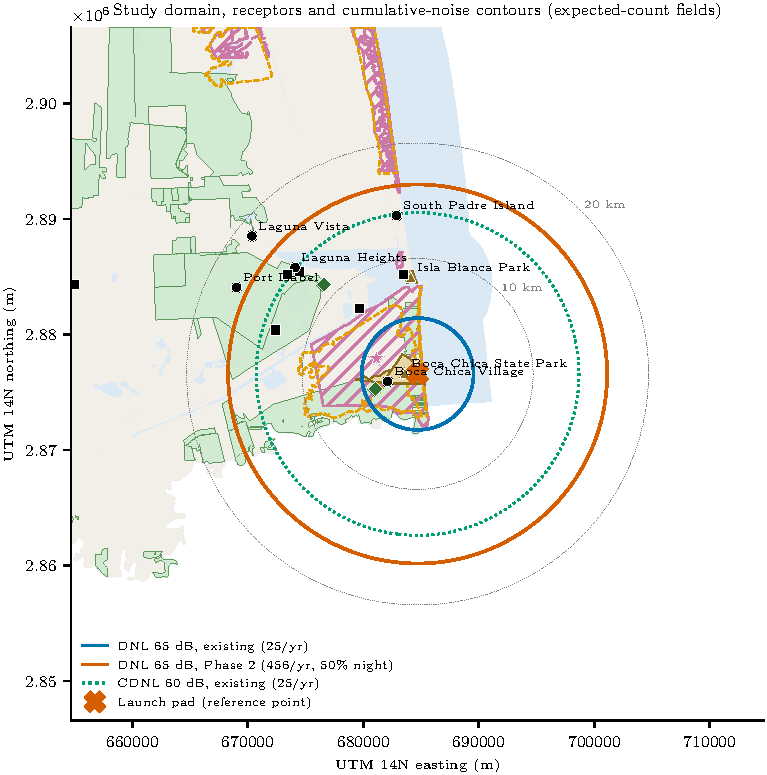
\includegraphics[width=0.85\textwidth]{fig1_site_map}
\caption{Study domain with receptors, refuges, critical habitat, parks and expected-count cumulative-noise contours (the existing-scenario $L_{dn}$ 65 dB and CDNL 60 dB contours and the Phase 2 $L_{dn}$ 65 dB contour).}
\label{fig:site}
\end{figure}

\subsection{Metric classes and closed forms}

Table~\ref{tab:metrics} lists the metric classes, their definitions and the Poisson closed forms used as test oracles, and Figure~\ref{fig:classes} sketches their scaling. For additive metrics $E[M] = \sum_\tau N_\tau \bar q_\tau$ exactly. For energy-averaged noise with fixed per-event levels, the change between two cadences is $10\log_{10}(N_2/N_1) + 10\log_{10}[(1+9f_{n,2})/(1+9f_{n,1})]$, where $f_n$ is the night fraction; from 25 to 456 launches with $f_n$ moving from 0.12 to 0.5 the terms are \valCfCountTermTwoFiveFourFiveSixDb~dB and \valCfNightTermZeroOneTwoZeroFiveDb~dB. The expected number of days with at least one event above $L$ among $D$ eligible days is $D(1 - e^{-N_L/D})$. For a receptor disturbed for an exponentially distributed recovery time with mean $\tau$ after each event, the stationary disturbed fraction is $\phi = 1 - \exp(-\lambda E[\tau])$ by the $M/G/\infty$ busy-period argument \citep{daley2003,hall1988}, which is linear in $\lambda$ only when $\lambda E[\tau] \ll 1$. Events are counted as disturbing a receptor when their $L_{A\max}$ exceeds 90~dBA or their boom exceeds 1~psf; recovery time and the required undisturbed window are swept over 1 min to 2 d and 1 h to 7 d, ranges that bracket resume-feeding times of seconds to minutes after pedestrian disturbance \citep{collop2016}, nest return within an hour after mobile pedestrian disturbance \citep{weston2011} and return to an area within hours after aircraft disturbance \citep{vanderkolk2020}; no species-specific value is asserted for the site. Coverage and interval metrics are evaluated over a season window of 1 March to 31 August, an illustrative six-month window for which no phenological claim is made.

\begin{figure}[htbp]
\centering
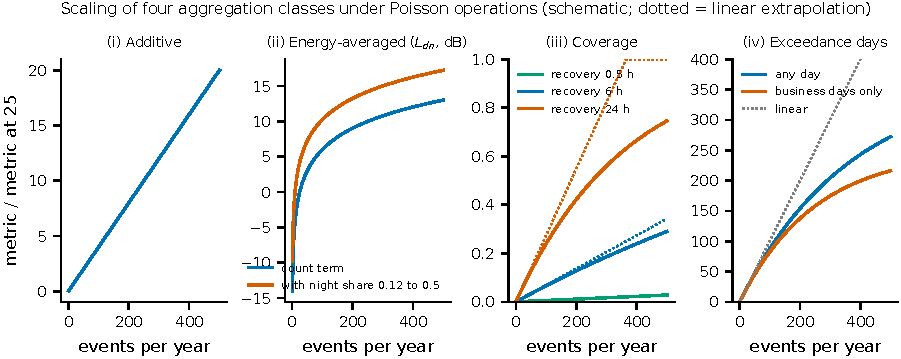
\includegraphics[width=\textwidth]{fig2_aggregation_classes}
\caption{Schematic scaling of the four aggregation classes under Poisson operations (closed forms with illustrative parameters; dotted lines are linear extrapolations).}
\label{fig:classes}
\end{figure}

\begin{table}[htbp]
\caption{Metric classes, definitions and Poisson closed forms.}
\label{tab:metrics}
\centering\scriptsize
\tableMetricDefinitions
\end{table}

\subsection{Aggregation error}

For a metric $Y$ and the reference cadence $N_0 = 25$, the linear-extrapolation error is $\varepsilon_Y(N) = [Y_{\mathrm{lin}}(N) - E[Y(N)]]/E[Y(N)]$ with $Y_{\mathrm{lin}}(N) = (N/N_0)\,E[Y(N_0)]$; for $L_{dn}$ the energy-average extrapolation error in decibels is reported. Bootstrap intervals over Monte Carlo realizations accompany each error.

\subsection{Sensitivity analysis}

Sixteen model inputs (night fraction, scrub probability, turnaround, number of pads, clustering rate and spread, level offset, boom factor, closure mean and dispersion, anomaly probability, static fires per launch, external landing fraction, share of Starship landings at the site, recovery time and window length) and the random-number seed of the realization are sampled uniformly over documented ranges (supporting information, Table S4) with a Saltelli design of $2^{13}$ base samples \citep{saltelli2010,sobol2001,herman2017}, giving \valESixNEvaluations~model evaluations per cadence. The seed is treated as a factor so that the same random numbers are used across the Saltelli matrices; Monte Carlo noise then appears as the seed's own index instead of inflating the total-order indices of the model inputs, and that index is the stochastic share of the output variance. Indices are computed at 25, 100 and 456 launches per year with campaign timing on business days, as first- and total-order indices with 200 bootstrap resamples for nine outputs; the implementation is verified against the analytical indices of the Ishigami function.

\subsection{Fleet emission inventory}

Annual emissions above the tropopause from methane--oxygen combustion for Starbase Phase 2 (456 launches), Launch Complex 39A (44 launches; \citealp{noaksc2026}) and Space Launch Complex 37 (76 launches; \citealp{rodslc37}) are $N\,M_{\mathrm{prop}}\,f_{\mathrm{strat}}\,\mathrm{EI}_s$ with propellant mass 6,000--6,750 t per launch from the 2025 assessment's stated capacities, a stratospheric fraction of 0.5--0.8 bracketing the two-thirds rule of \citet{ross2014} and the 78--79\% above 15 km of \citet{ryan2022}, and emission indices for H$_2$O, CO$_2$, CO, NO$_x$ and black carbon from \citet{barker2024}, \citet{ross2014}, \citet{ryan2022} and \citet{tsigaridis2024}. No atmospheric chemistry or transport is modelled; black carbon is compared with the 10, 30 and 100 Gg/yr scenarios of \citet{maloney2022}.

\subsection{Computation and reproducibility}

Each configuration uses \valMcNRealizations~annual realizations with seeds spawned from one seed sequence. The Monte Carlo standard error of every headline quantity is below \valMcMaxSeFractionPct\% of its value. Grid convergence between 250 m and 125 m cells changes the Phase 2 contour areas by at most \valConvPhaseTwoMaxRelPct\% and the verification-scenario areas by at most \valConvVerifMaxRelPct\%. All inputs, code, configurations and outputs are in the companion repository; one command regenerates every number and figure.

\section{Results}
\label{sec:results}

\subsection{Verification against the 2025 assessment}

Table~\ref{tab:verif} compares quantities stated in the 2025 assessment with their reproduction from the per-operation inputs. With 22 daytime and 3 night launches, 22 daytime landings of each vehicle and 11 static fires, the $L_{dn}$ 65 dB contour extends \valVerifDnlSixFiveDbContourExtentMiles~miles against 3 to 3.5 miles stated in the noise appendix and \valVerifDnlSixFiveDbOverlandContourRadiusDigitizedFigureTwoOneMiles~miles digitized from its DNL map; the CDNL 60 dB contour from 44 daytime booms extends \valVerifCdnlSixZeroDbContourExtentMiles~miles against approximately 5 miles stated; the annual emission totals are reproduced exactly by construction. The DNL extent agrees with the digitized map to within 0.1 mile; the CDNL extent is about 20\% larger than the stated extent; the boom law is isotropic and fitted to the maximum contour extents stated in the assessment, whereas the modelled boom footprints are directional, so an overstatement in this direction is expected. Both involve the digitized footprints, the day/night weighting and the FAA conversion from overpressure to C-weighted level, and together they establish model verification at the level of the conceptual model used by the agency.

\begin{table}[htbp]
\caption{Verification against values stated in the 2025 Tiered Environmental Assessment.}
\label{tab:verif}
\centering\footnotesize
\tableVerification
\end{table}

\subsection{Scaling of each metric class with cadence}

Figure~\ref{fig:scaling} shows nine metrics against cadence under Poisson timing with half of operations at night, and Table~\ref{tab:errors} gives the aggregation errors at 456 launches per year. Additive totals, number-above counts and boom counts scale linearly within Monte Carlo error, and $L_{dn}$ at the Port Isabel edge follows the energy-average closed form to within \valEThreeNightCfMaxabsdiffDb~dB. Exceedance days depart strongly: at the South Padre Island edge, where launches and both landing types exceed 90~dBA, the expected number of days with an event is \valEOneSimDaysNineZeroSouthPadreIslandNearestEdge~at 456 launches per year against \valEOneNTwoFiveDaysNineZeroSpi~at 25, so linear extrapolation overstates the day count by \valEOneRelerrPctDaysNineZeroSouthPadreIslandNearestEdge\% and the quantity that grows at high cadence is the number of events per exposed day, not the number of exposed days. Closure hours for operations (excluding anomaly response) are sublinear because windows overlap (\valEOneSimClosureH~h simulated against \valEOneLinClosureH~h extrapolated), but remain far above every cap considered. Weekend and holiday daylight availability falls from \valEOneNTwoFiveWeekendAvail~to \valEOneNFourFiveSixWeekendAvail~of hours as cadence rises, a quantity with no per-operation analogue. The disturbed fraction at the habitat receptor with a one-hour recovery time remains close to linear at 456 launches per year because $\lambda E[\tau]$ is still small; its saturation is governed by the recovery time (Section~\ref{sec:coverage}). Allowing landings of vehicles launched elsewhere up to the 912 per year analysed in the notice raises the number of booms above 1~psf at the Port Isabel edge from \valEOneExtBoomOnePortisabelZero~to \valEOneExtBoomOnePortisabelOne~per year and the days above 90~dBA at South Padre Island from \valEOneExtDaysNineZeroSpiZero~to \valEOneExtDaysNineZeroSpiOne, while changing $L_{dn}$ by \valEOneExtLdnDeltaDb~dB.

\begin{figure}[htbp]
\centering
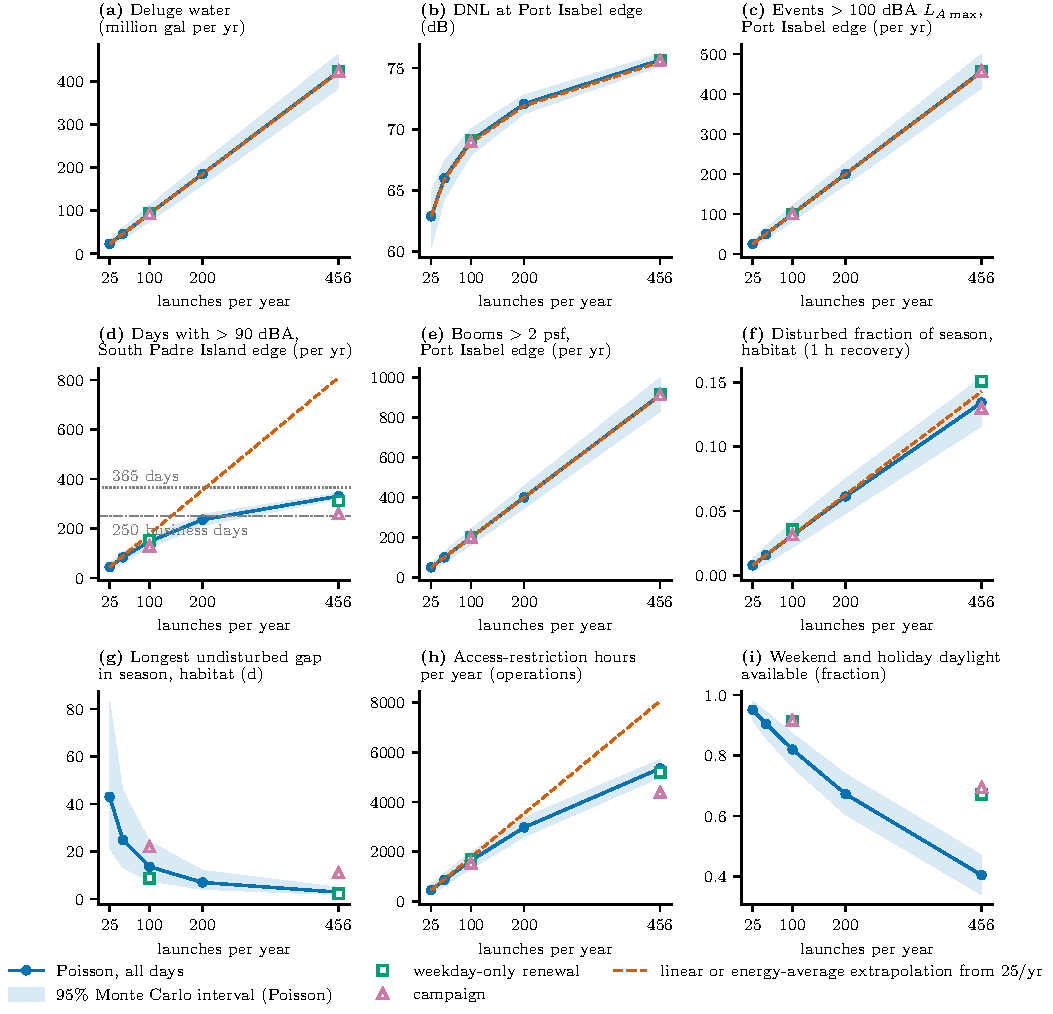
\includegraphics[width=\textwidth]{fig3_metric_vs_cadence}
\caption{Metrics against cadence under Poisson timing with half of operations at night and no landings of externally launched vehicles. Shaded bands are 95\% Monte Carlo intervals; dashed lines are linear (or energy-average) extrapolations from 25 launches per year. Closure parameters other than the launch-window mean are hypothetical.}
\label{fig:scaling}
\end{figure}

\begin{table}[htbp]
\caption{Aggregation errors at 456 launches per year relative to extrapolation from 25 (Poisson timing, 50\% night).}
\label{tab:errors}
\centering\scriptsize
\tableAggregationErrors
\end{table}

\subsection{Night share and contour expansion}

The night-share term of the $L_{dn}$ closed form is reproduced by simulation to within \valEThreeNightCfMaxabsdiffDb~dB across night fractions from 0 to 0.5. Figure~\ref{fig:maps} maps the expected-count $L_{dn}$ field at 25, 100 and 456 launches per year. The $L_{dn}$ 65 dB area grows from \valAreaExistingLdnSixFiveKmTwo~km$^2$ (existing, 12\% night) to \valAreaPhaseOneLdnSixFiveKmTwo~km$^2$ (Phase 1) and \valAreaPhaseTwoLdnSixFiveKmTwo~km$^2$ (Phase 2, 50\% night); at 456 launches with the existing 12\% night share the area would be \valAreaPhaseTwoFnZeroOneTwoLdnSixFiveKmTwo~km$^2$, so the night-share assumption accounts for the difference between those two figures. The 2020 census population within the maximum $L_{dn}$ 65 dB extent is \valPopLdnSixFiveExisting~for the existing scenario and \valPopLdnSixFivePhaseTwo~for Phase 2; these are expected-count fields from the FAA's single-event contours, not the PEIS noise model, and the counts are reported to show the sensitivity of a population metric to the night share rather than as an impact estimate. The expected-count CDNL field from 912 booms per year with half at night exceeds 60~dB throughout the 60 km domain, since the 44-boom CDNL 60 dB extent of about 5 miles moves outward by $10\log_{10}(912/44)$ plus the night term; the digitized boom footprints do not extend beyond 28 miles, so this statement is bounded by the domain and the extrapolated boom law. At 456 launches per year the number of night-time events above 100~dBA at the Port Isabel edge is \valEThreeNaOneZeroZeroNightPortisabelFnFiveZero~with half of operations at night against \valEThreeNaOneZeroZeroNightPortisabelFnOneTwo~with the existing night share.

\begin{figure}[htbp]
\centering
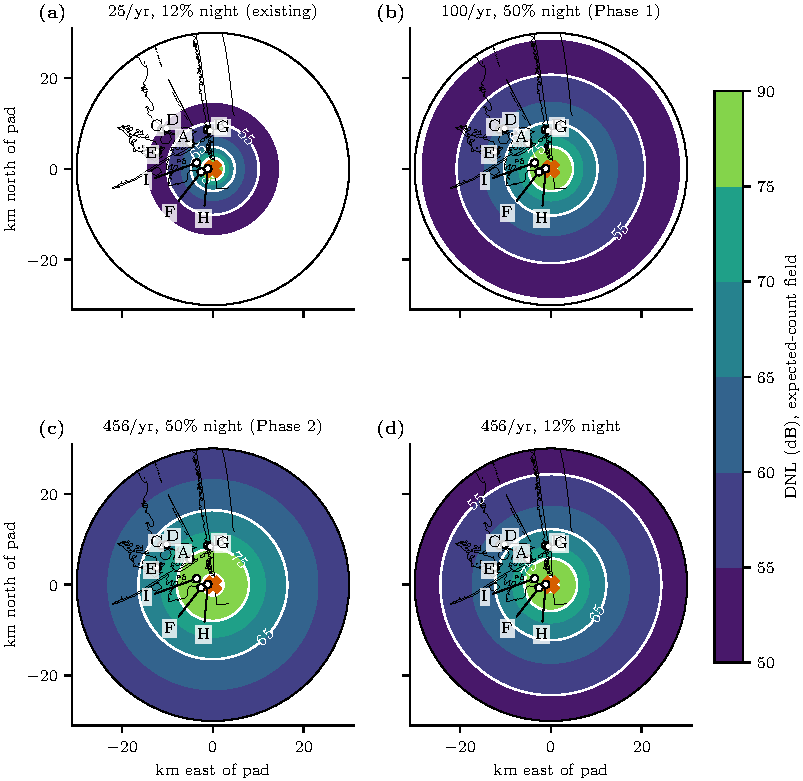
\includegraphics[width=\textwidth]{fig4_ldn_maps}
\caption{Expected-count $L_{dn}$ fields from the digitized single-event SEL footprints at the existing, Phase 1 and Phase 2 cadences, and Phase 2 with the existing night share. Community receptors are shown as dots.}
\label{fig:maps}
\end{figure}

\subsection{Temporal clustering and the weekday restriction}

At fixed annual count, the temporal model changes the interval and availability metrics but not the additive, energy-averaged or number-above metrics (Table S5). At 456 launches per year the weekday renewal model gives \valETwoWeekdayDaysNineZeroSpi~exposure days at the South Padre Island edge against \valETwoPoissonDaysNineZeroSpi~under Poisson timing, because launches and booster landings are confined to the 250 business days and only the Starship landings that follow spill into weekends; the campaign model gives \valETwoCampaignDaysNineZeroSpi. Weekend daylight availability is \valETwoWeekdayWeekendAvail~under the weekday model against \valETwoPoissonWeekendAvail~under Poisson timing, because landings and the tails of closure windows still fall on weekends even when launches do not. The longest undisturbed gap at the habitat receptor within the season window is \valETwoPoissonLongestGapHabitatH~h (Poisson), \valETwoWeekdayLongestGapHabitatH~h (weekday) and \valETwoCampaignLongestGapHabitatH~h (campaign), while a four-hour undisturbed window occurs in every realization under all three models; clustering redistributes rather than removes undisturbed time. The ranking of the cadence scenarios on every metric is unchanged across temporal models, so hypothesis H2 in its strong form (that the metric choice changes which scenario appears most affected) is not supported, while the magnitudes of the interval metrics do depend on the temporal model.

\subsection{Closure caps and cadence}
\label{sec:closures}

Figure~\ref{fig:closures} shows the distribution of annual access-restriction hours under three per-launch closure distributions bracketing the FAA record, and Table S6 gives the probability of exceeding 500, 800 and 2,000 h. With the mean of the Flight 1--4 record (\valRecordMeanLaunchClosureH~h per launch campaign) and hypothetical allocations for other events, the expected annual hours including anomaly response (hypothetical probability 0.02 per launch, 48 h each) are \valEFourRecordFlightsOneToFourNOneZeroZeroClosureH~h at 100 launches and \valEFourRecordFlightsOneToFourNFourFiveSixClosureH~h at 456, with $P(H > 2000) = \valEFourRecordFlightsOneToFourNFourFiveSixPexceedTwoZeroZeroZero$ at 456 launches per year. The budget implied by the caps is \valBudgetPerLaunchTwoZeroZeroZeroNFourFiveSixH~h per launch for 2,000 h at 456 launches and \valBudgetPerLaunchFiveZeroZeroNFourFiveSixH~h for 500 h, against 7.75 h for the shortest recorded launch. Applying the 2022 PEA measures (no closures on listed holidays or summer weekends) to the Phase 2 weekday schedule leaves \valEFourRecordWeekdayPhaseTwoPeaMeasuresNFourFiveSixSummerAvail~of summer daylight hours available against \valEFourRecordWeekdayPhaseTwoNFourFiveSixSummerAvail~without them. Whether the 2,000-hour assumption is consistent with the proposed cadence therefore depends on a per-launch closure duration well below the shortest value in the public record, a quantity the PEIS can state.

\begin{figure}[htbp]
\centering
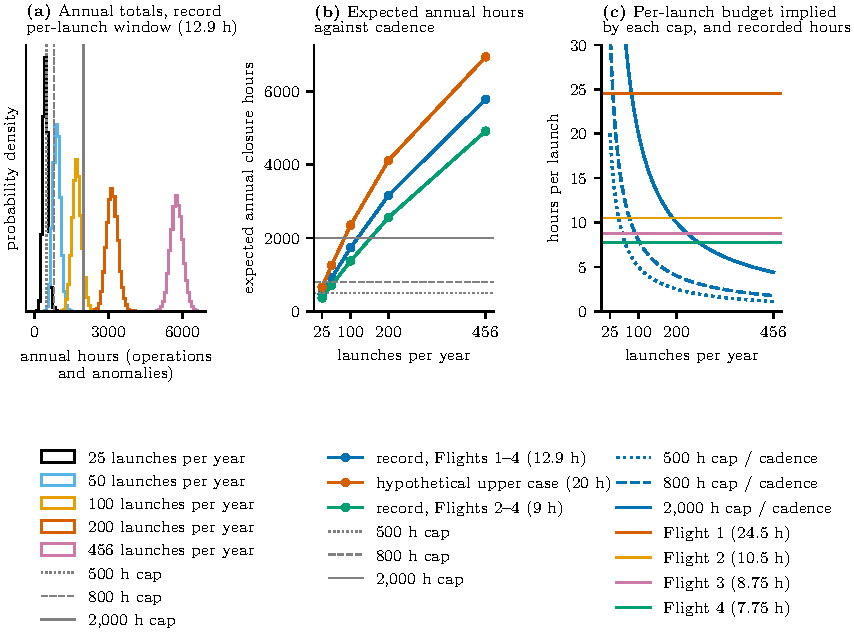
\includegraphics[width=\textwidth]{fig6_closure_distributions}
\caption{Annual access-restriction hours: Monte Carlo distributions under the record-based per-launch distribution (left), expected hours against cadence for three distributions (centre) and the per-launch budget implied by each cap compared with the recorded per-launch hours (right).}
\label{fig:closures}
\end{figure}

\subsection{Disturbance-coverage regimes}
\label{sec:coverage}

Figure~\ref{fig:coverage} maps the disturbed fraction, the linear-extrapolation error and the probability that no undisturbed window of length $w$ occurs in the season at the piping plover critical-habitat receptor, over recovery times from 1 min to 2 d. The simulated disturbed fraction follows the Poisson closed form $1 - e^{-\lambda E[\tau]}$ to within \valEOneCoverageCfMaxabsdiff~in absolute terms, the simulated value lying below the closed form because booster landings follow launches within minutes and static fires precede them, so that the events are not independent. The linear (per-event) extrapolation overstates the simulated coverage by more than 10\% for recovery times of about \valEFiveWeekdayTauOneZeroPctH~h or longer at 456 launches per year under weekday timing (disturbing-event rate \valEFiveWeekdayRatePerDayNFourFiveSix~per day at this receptor), partly through the saturation of the closed form and partly through this pairing of events. With a one-hour recovery time the disturbed fraction is \valEFiveWeekdayDisturbedTauOneH; with one day it is \valEFiveWeekdayDisturbedTauTwoFourH. With a one-day recovery time the probability that the season contains no undisturbed window of one day is \valEFiveWeekdayHaswindowComplementWOneDayTauTwoFourH; with a one-hour recovery time it is \valEFiveWeekdayHaswindowComplementWOneDayTauOneH. These are response surfaces in two unknown parameters, not species-specific predictions; the location of the site's receptors on the surface is the quantity the PEIS would need to establish.

\begin{figure}[htbp]
\centering
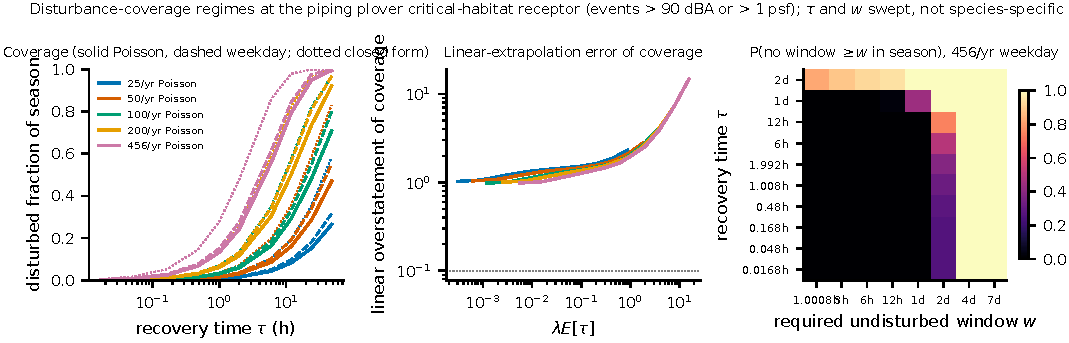
\includegraphics[width=\textwidth]{fig5_coverage_surfaces}
\caption{Coverage and interval metrics at the piping plover critical-habitat receptor as functions of recovery time and required window, for Poisson and weekday timing at five cadences. Dotted lines are the Poisson closed form.}
\label{fig:coverage}
\end{figure}

\subsection{Dominant uncertainties}

Figure~\ref{fig:sobol} shows total-order Sobol indices by output, input and cadence; Table S7 lists factors with $S_T > 0.05$. At 456 launches per year the hypothetical vehicle-variant level offset dominates $L_{dn}$ and the number of events above 100~dBA (top factor \valESixTopLdnNFourFiveSix, $S_T = \valESixTopstLdnNFourFiveSix$ for $L_{dn}$ and \valESixTopstNaOneZeroZeroNFourFiveSix~for the count), with the night fraction second for $L_{dn}$ at every cadence; night share and the boom factor share the CDNL variance almost equally; the external landing fraction dominates boom counts, exceedance days and the longest undisturbed gap, with the campaign rate second for the last two; the recovery time dominates the disturbed fraction ($S_T = \valESixTopstDisturbedNFourFiveSix$); and the closure-window mean dominates closure hours (with the anomaly probability second) and weekend availability (with the scrub probability second). The index of the random seed is the share of variance due to Monte Carlo variation of a single simulated year; at 456 launches per year it is at most 0.2 for every output except the boom count and the longest gap, whose single-year values are the most variable, and at 25 launches per year it is the largest index for the exceedance-day, boom-count, longest-gap and weekend-availability outputs, so that at the existing cadence year-to-year variation exceeds the effect of any input on those four metrics. Hypothesis H3, that divergence between per-event and cumulative assessment for biological receptors depends mainly on unknown recovery parameters, is supported for the coverage metrics; for the community noise and access metrics the dominant uncertainties are operational choices (night share, closure practice, vehicle configuration) that the applicant and agency can state.

\begin{figure}[htbp]
\centering
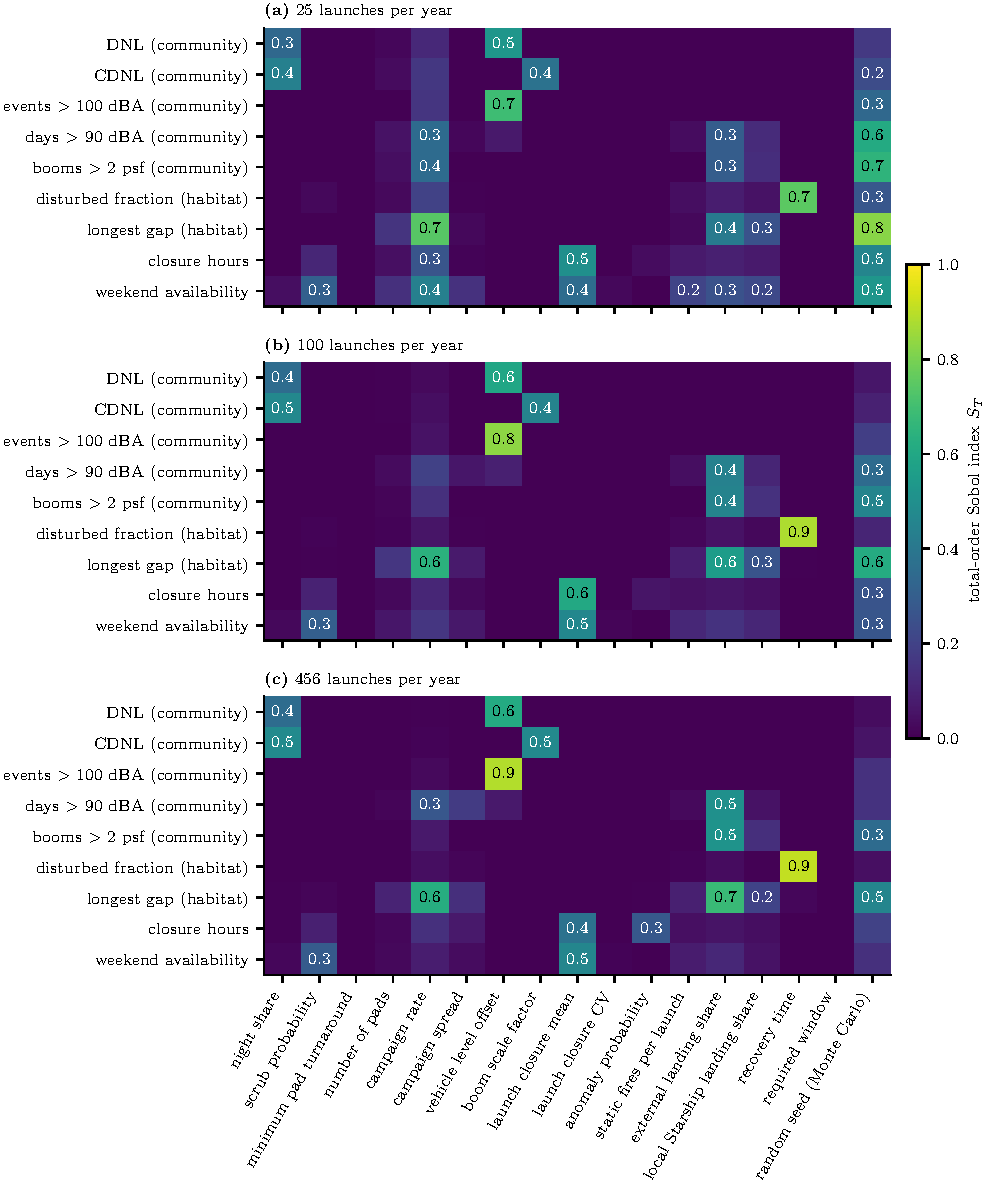
\includegraphics[width=\textwidth]{fig7_sobol_heatmap}
\caption{Total-order Sobol indices for nine outputs and sixteen inputs at three cadences (campaign timing on business days). Inputs are sampled over the ranges in Table S4; hypothetical ranges are identified there.}
\label{fig:sobol}
\end{figure}

\subsection{Footprint scaling and fleet emissions}

For a hypothetical louder vehicle variant (+6 dB on all levels, 1.5 times the boom overpressure) at 456 launches per year, the $L_{dn}$ 65 dB area is \valESevenNFourFiveSixOffSixBsOneFiveLdnSixFiveArea~km$^2$ against \valESevenNFourFiveSixOffZeroBsOneZeroLdnSixFiveArea~km$^2$ at the digitized levels, and the area receiving more than ten booms above 2~psf per year is \valESevenNFourFiveSixOffSixBsOneFiveBoomTwoArea~km$^2$ against \valESevenNFourFiveSixOffZeroBsOneZeroBoomTwoArea~km$^2$, both bounded by the 3,600 km$^2$ domain. The fleet inventory (Table S8) gives median annual black-carbon emissions above the tropopause of \valEEightFleetTotalBcMedianT~t (5th to 95th percentile \valEEightFleetTotalBcPZeroFiveT--\valEEightFleetTotalBcPNineFiveT~t) for \valEEightFleetLaunches~launches per year across the three sites, which is \valEEightBcFleetOverOneZeroGgMedian~of the 10 Gg/yr scenario of \citet{maloney2022}, and median H$_2$O of \valEEightFleetTotalHTwoOMedianT~t; the width of the intervals reflects the absence of measured emission indices for methane engines.

\section{Discussion}
\label{sec:discussion}

The results separate three groups of metric. Additive, number-above and energy-averaged metrics scale as their closed forms predict, so a per-operation assessment extrapolates to any cadence once the count and night share are stated; the question for such metrics is only whether the per-event footprint is right. Exceedance-day, availability and closure metrics saturate or interact, so the quantity that characterizes high cadence is not the one that characterized low cadence: days with an event become nearly every eligible day, and the informative quantities become events per exposed day, hours of weekend daylight closed, and the per-launch closure budget implied by any cap. Coverage and interval metrics for disturbance-sensitive receptors sit between the two groups, with their regime set by $\lambda E[\tau]$; the framework turns a question about impacts into a question about one measurable product.

Three consequences follow for programmatic reviews of growing operations. First, the metric set should include at least one member of each aggregation class, because no single class distinguishes the cadence scenarios on all dimensions: $L_{dn}$ separates 25 from 456 launches by \valCfTotalTwoFiveFourFiveSixDb~dB; exceedance days at the South Padre Island edge rise only from \valEOneNTwoZeroZeroDaysNineZeroSpi~to \valEOneNFourFiveSixDaysNineZeroSpi~between 200 and 456 launches, a far smaller ratio than the count; and weekend daylight availability falls from \valEOneNTwoZeroZeroWeekendAvail~to \valEOneNFourFiveSixWeekendAvail~over the same interval. Hypothesis H1 therefore holds for the first group of metrics and fails for the second; H2 holds for the magnitudes of the interval metrics but not for the ranking of scenarios; H3 holds for the biological coverage metrics and not for the community noise and access metrics. Second, the temporal distribution of operations should be stated and analysed, not only the annual count, because interval metrics depend on it while count-based metrics do not; the weekday restriction in the notice of intent is such a statement, and the results show which metrics it affects. Third, the parameters that control each metric differ, so sensitivity analysis can be targeted: night share and vehicle configuration for noise, closure practice for access, recovery times for biological coverage. For biological receptors the dominant unknown is the recovery time, and the most valuable measurement would be the return time of the species of concern after a launch or landing at this site. The only published launch-site return time found is for pinnipeds at Vandenberg, where harbor seals displaced by Titan IV launch noise returned to land within several hours \citep{stewart1993}; no return time has been published for shorebirds at any launch site.

The framework applies to any repeated-disturbance source: airports with growing operations, pile driving, military ranges and construction sequences. Its inputs are per-event footprints and a calendar model; its outputs are the scaling laws and errors reported here.

\section{Limitations}

The per-event footprints are the FAA's modelled contours for the vehicle configuration assessed in 2024, digitized from maps with the residuals reported; they are not measurements and may not describe future configurations, which the scaling-factor experiment addresses only parametrically. The footprints depend on distance only, using the overland-sector median radius of each digitized contour, so the modelled contours are circular where the FAA contours are directional, and areas and populations within contours are those of the circular fields. Future operational patterns within the stated caps are unknown; the temporal models bracket them with hypothetical parameters. Species-specific recovery times and required windows at the site are unknown; the coverage results are conditional response surfaces. No validation of ecological response is possible from public data. The closure record consists of four per-launch values stated in the 2025 assessment; a complete official record could not be compiled because the county notice archive is no longer served, and the closure results therefore rest on a parameterized distribution bracketing those values. The emission inventory carries wide intervals because emission indices for methane engines have not been measured. None of the results estimates the actual impact of the proposed action.

\section{Conclusions}

A marked point-process model of operations with a taxonomy of metrics by aggregation operator makes explicit which cumulative-effect metrics scale linearly with operating frequency and which do not. Applied to the cadence scenarios of the Boca Chica PEIS with the FAA's own per-event inputs, and verified against the agency's 2025 cumulative-noise results, the model shows that energy-averaged and count metrics extrapolate as their closed forms predict, that exceedance-day, availability and closure metrics saturate or interact, and that the behaviour of disturbance-coverage metrics is set by the product of event rate and recovery time. The annual access-restriction hours implied by the recorded per-launch closure durations exceed the 2,000-hour assumption at the proposed cadence unless per-launch durations fall well below the shortest value in the record. These findings identify which metrics, temporal information, sensitivity analyses and measurements a programmatic review of high-cadence operations needs; they do not estimate impacts.

\section*{Data and code availability}
All code, configurations, transcribed inputs, digitized contours and generated outputs are in the repository \texttt{launch-cumulative-screening}; one command reproduces every number and figure.

\section*{Declaration of competing interest}
The author declares no competing interests.

\section*{Funding}
This research received no specific grant from any funding agency in the public, commercial, or not-for-profit sectors.

\bibliographystyle{elsarticle-harv}
\bibliography{references}

\end{document}
